\documentclass[11pt]{article}
\usepackage[utf8]{inputenc}
\usepackage[dvipsnames]{xcolor}
\usepackage{tikz}
\usepackage{enumitem}
\usepackage{hhline}
\usepackage{fancyvrb}
\topmargin=-0.45in
\evensidemargin=0in
\oddsidemargin=0in
\textwidth=6.5in
\textheight=9.0in
\headsep=0.25in
\begin{document}

\begin{titlepage}
    \begin{center}
        \begin{tikzpicture}[remember picture,overlay]
            \node[anchor=north west,yshift=-1.5pt,xshift=1pt]%
            at (current page.north west)
            {
\includegraphics[scale=1]{ethlogo.pdf}};
        \end{tikzpicture}
        \begin{tikzpicture}[remember picture,overlay]
              \node[anchor=north east,inner sep=0pt, xshift=-0.2cm] at (current page.north east)
              {
\includegraphics[scale=0.4]{systems-logo.pdf}};
        \end{tikzpicture}

            
        \Huge
        \textbf{Cloud computing architecture}
            
        \vspace{0.5cm}
        \LARGE
        Semester project report
            
        \vspace{1.5cm}
            
        \textbf{Group 027}
            
        Jiale Chen - 20-961-504 \\
        Ran Liao - 20-949-186 \\
        Xintian Yuan - 20-951-778 \\
        \vfill
            
            
        \Large
        Systems Group\\
        Department of Computer Science\\
        ETH Zurich\\
        \today
            
    \end{center}
\end{titlepage}
\section*{Instructions}
Please do not modify the template, except for putting your solutions, names and legi-NR.
%Parts 3 and 4 should be answered in maximum 10 pages (including the questions).
%\textbf{If you exceed the space, points might be subtracted}.
\newpage
\section*{Part 3 [34 points]}
\begin{enumerate}
    \item \textbf{[17 points]} With your scheduling policy, run the entire workflow 3 separate times. For each run, measure the execution time of each PARSEC job, as well as the latency outputs of memcached running with a steady client load of 30K QPS. For each PARSEC application, compute the mean and standard deviation of the execution time across three runs. Also compute the mean and standard deviation of the total time to complete all jobs. Fill in the table below. Finally, compute the SLO violation ratio for memcached for the three runs; the number of datapoints with 95th percentile latency $>$ 2ms, as a fraction of the total number of datapoints.  Do three plots (one for each run) of memcached p95 latency (y-axis) over time (x-axis) with annotations showing when each parsec job started.
    
    \textbf{Solution:}
    
    The SLO violation ratio for all three runs are 0. The orange line annotates when each PARSEC job starts. The plots are only drawn to the point where all PARSEC jobs finished.
    
    \begin{table}[h]
\centering
\begin{tabular}{ |c|c|c|c|c|} 
\hline
job name & mean time [s] & std [s] \\ \hline \hline
dedup         & 53.67 & 0.94 \\  \hline
blackscholes  & 195.67 & 1.25\\  \hline
ferret        & 261 & 6.38 \\  \hline
freqmine      & 267 & 8.52 \\  \hline
canneal       & 278 & 12.75 \\  \hline
fft           & 144.67 & 12.97\\  \hline
total time    & 280.33 & 13.22\\ \hline
\end{tabular}
\end{table}
    
    \begin{center}
    {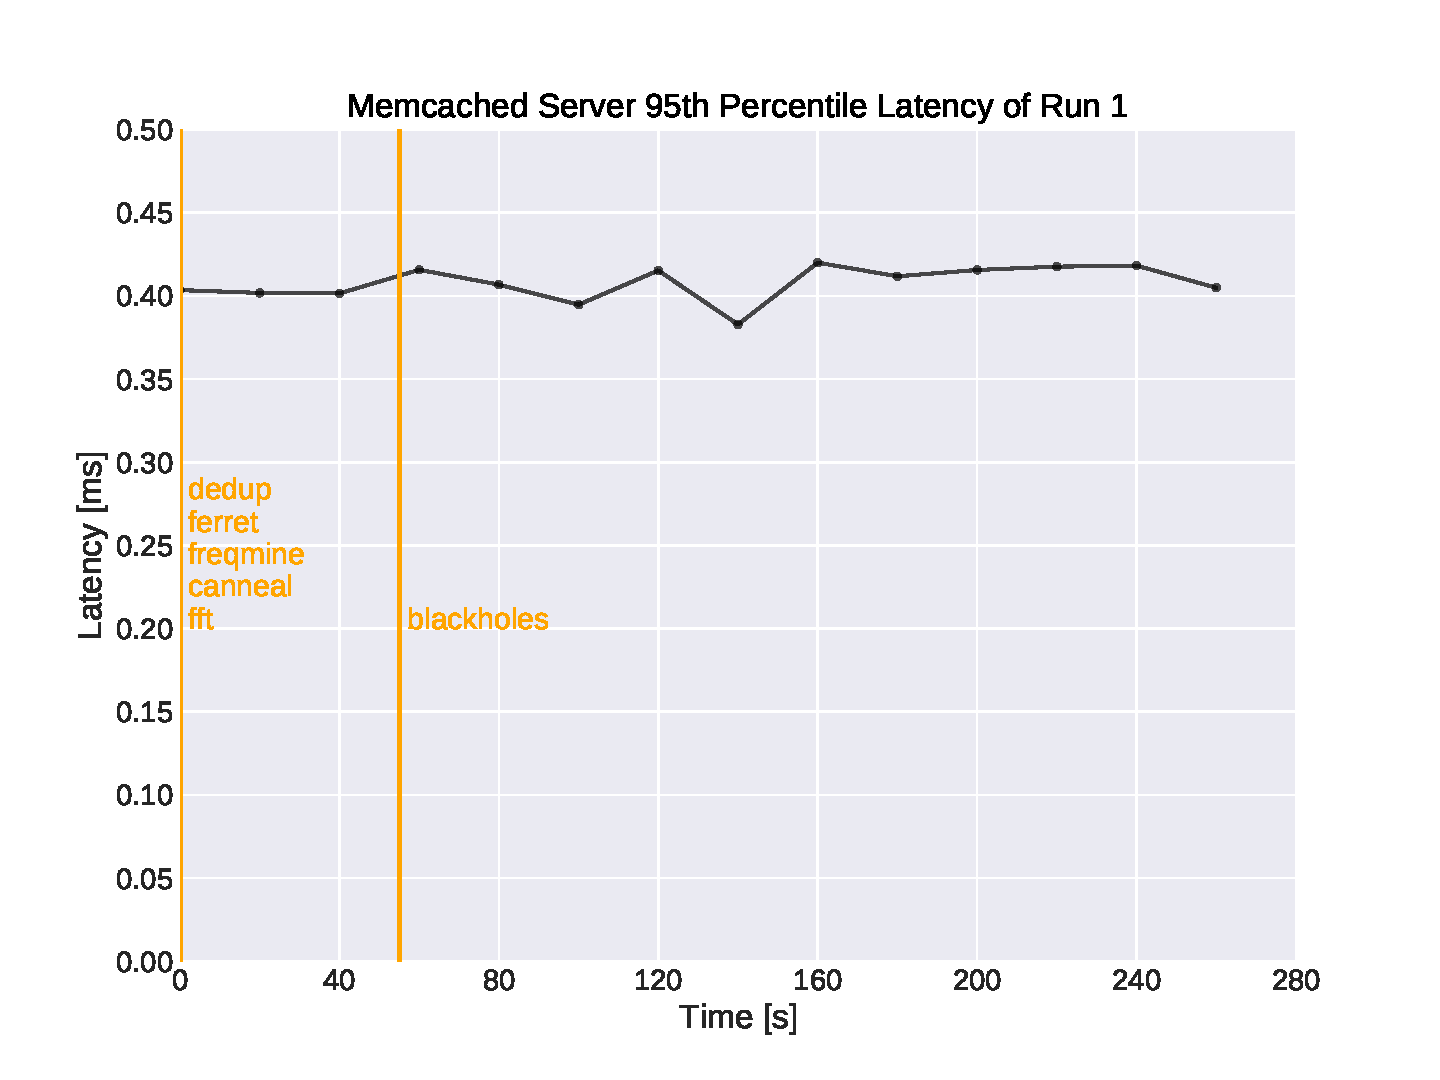
\includegraphics[width=0.9\textwidth]{m4.pdf}}
    \end{center}
    \begin{center}
    {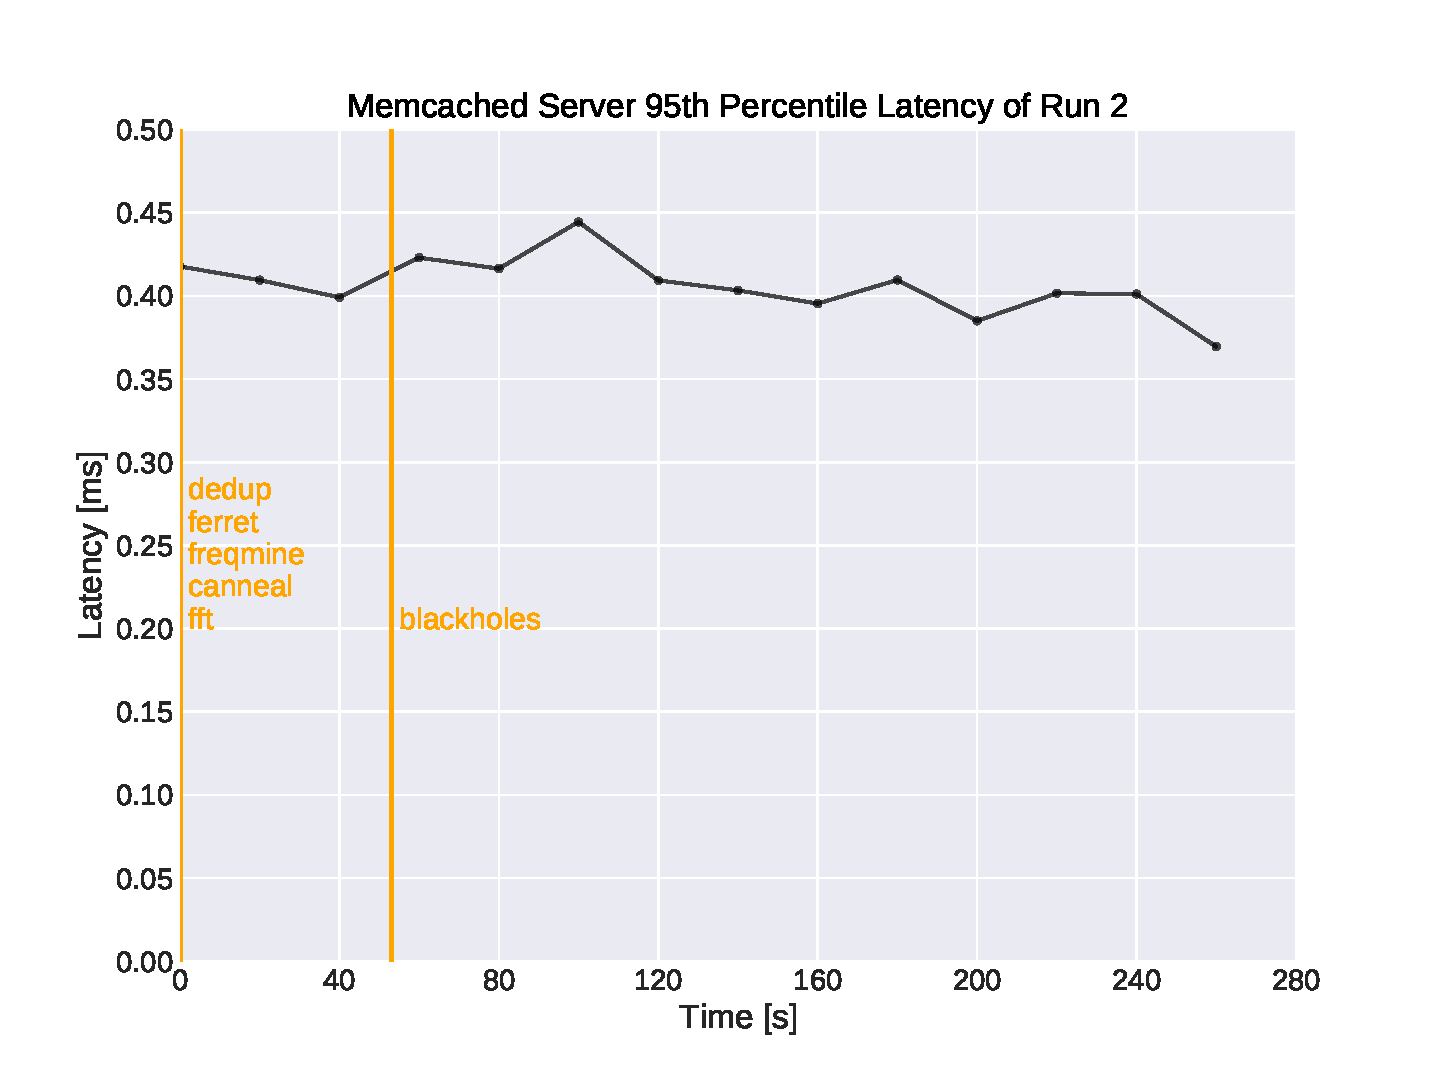
\includegraphics[width=0.9\textwidth]{m5.pdf}}
    \end{center}
    \begin{center}
    {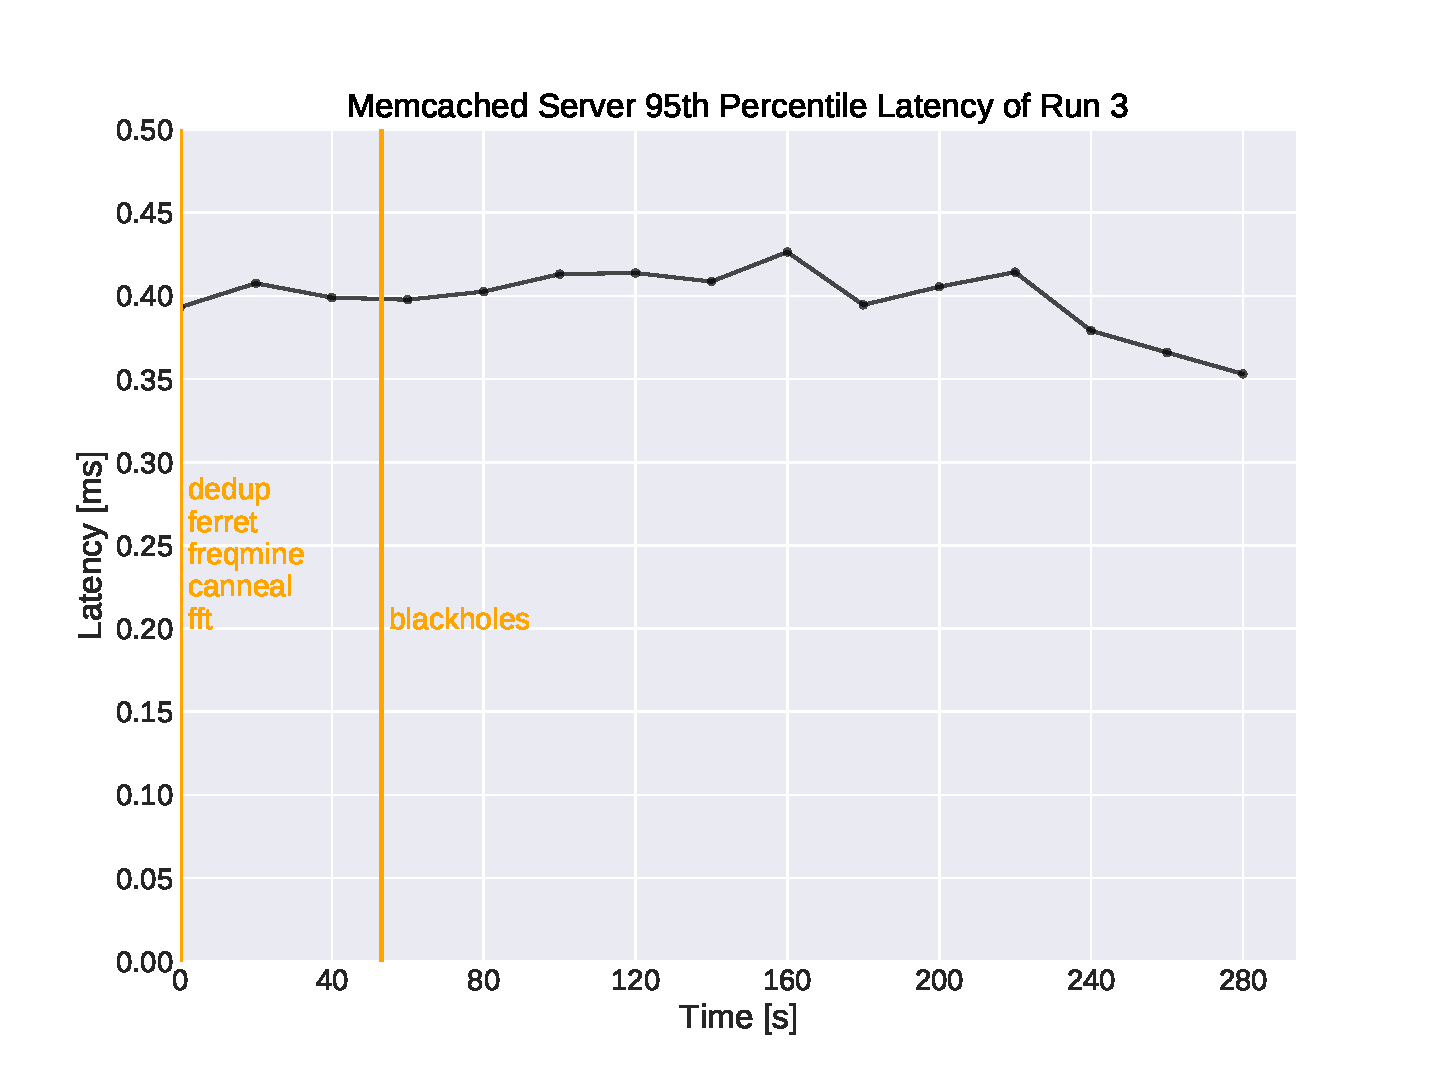
\includegraphics[width=0.9\textwidth]{m6.pdf}}
    \end{center}

    \item \textbf{[17 points]} Describe and justify the “optimal” scheduling policy you have designed. This is an open question, but you should at minimum answer the following questions: 
    \begin{itemize}
        \item	Which node does memcached run on?
        \item	Which node does each of the 6 PARSEC apps run on? 
        \item	Which jobs run concurrently / are collocated?
        \item	In which order did you run 6 PARSEC apps?
        \item	How many threads you used for each of the 6 PARSEC apps? 
    \end{itemize}
    Describe how you implemented your scheduling policy. Which files did you modify or add and in what way? Which Kubernetes features did you use? Please attach your modified/added YAML files, run scripts and report as a zip file.
    \textbf{Important: The search space of all the possible policies is exponential and you do not have enough credit to run all of them. We do not ask you to find the policy that minimizes
    the total running time, but rather to design a policy that has a reasonable running time, does not violate the SLO and takes into account the characteristics of the first two parts of the project.}
    
    \textbf{Solution:}
    
    
    Our solution distributed the seven jobs (one memcached and 6 PARSEC) on different nodes with various cores. We use nodeSelector to run jobs only on specified node. We use taskset to restrict each job only running on specified cpu cores. See the following table for details.

\begin{table}[h]
\centering
\begin{tabular}{ |c|c|c|c|c|} 
\hline
job name & node & cpu id & number of threads \\ \hline \hline
dedup         & 2-cores-node & 0-1 & 2\\  \hline
blackscholes  & 2-cores-node & 0-1 & 2\\  \hline
freqmine      & 4-cores-node & 0-3 & 4\\  \hline
fft           & 4-cores-node & 0-3 & 4\\  \hline
memcached     & 8-cores-node & 0   & 1\\  \hline
ferret        & 8-cores-node & 1-7 & 7\\  \hline
canneal       & 8-cores-node & 4-7 & 4\\  \hline
\end{tabular}
\end{table}

    At first, dedup, ferret, freqmine, canneal and fft starts simultaneously and runs concurrently, then blackscholes will start after dedup is completed. 
    This means memcached, canneal and ferret are collocated on 8-cores-node. 
    At the same time fft and freqmine are collacted on core 4-cores-node. 
    But dedup and blackscholes will not collcated with each other and will run sequentially. 
    We used blackscholes with 2 threads, canneal with 4 threads, dedup with 2 threads, ferret with 7 threads, fft with 4 threads and freqmine with 4 threads(1 thread for each cpu core they can use). 
    We modified the respective YAML file to the configuration mentioned above and add a scheduler.py python script to automate the scheduling process.
    
    We put memcached into the 8-cores-node because from part 2.3 we learned that all PARSEC jobs are sub-linear with more than 4 threads. This means give a job with 7 threads or 8 threads doesn't make much difference. In 8-cores-node machine, memcached will use 1 core, but we still can execute jobs on the remaining 7 cores. ferret is quite time consuming among all PERSEC jobs and become the bottleneck somehow. So we run it with 7 threads, this is almost the maximum possible resource we can allocate to this job.
    
    And to maximize resource utilization, we try to let jobs in 2-cores-node, 4-cores-node and 8-cores-node complete approximately the same time.
    
\end{enumerate}

\newpage

\section*{Part 4 [76 points]}

\begin{enumerate}
\itemsep 2em
    \item \textbf{[10 points]} How does memcached performance vary with the number of threads ($T$) and number of cores ($C$) allocated to the job? In a single graph, plot the 95th percentile latency (y-axis) vs. QPS (x-axis) of memcached (running alone, with no other jobs collocated on the server) for the following configurations (one line each):
    \begin{itemize}
        \item Memcached with $T$=1 thread, $C$=1 core
        \item Memcached with $T$=1 thread, $C$=2 cores
        \item Memcached with $T$=2 threads, $C$=1 core
        \item Memcached with $T$=2 threads, $C$=2 cores
    \end{itemize}
    
    For this question, use the following \texttt{mcperf} command to vary QPS from 5K to 120K: 
    \begin{Verbatim}[fontsize=\small]
$ ./mcperf -s INTERNAL_MEMCACHED_IP --loadonly 
$ ./mcperf -s INTERNAL_MEMCACHED_IP -a INTERNAL_AGENT_IP  \
           --noload -T 16 -C 4 -D 4 -Q 1000 -c 4 -t 5 \ 
           --scan 5000:120000:5000
\end{Verbatim}

    Label the axes in your plot. State how many runs you averaged across (we recommend three runs) and include error bars. The readability of your plot will be part of your grade.
    
    What do you conclude from the results in your plot? Summarize in 2-3 brief sentences how memcached performance varies with the number of threads and cores. 
    
    \textbf{Solution:}
    
    \begin{center}
    {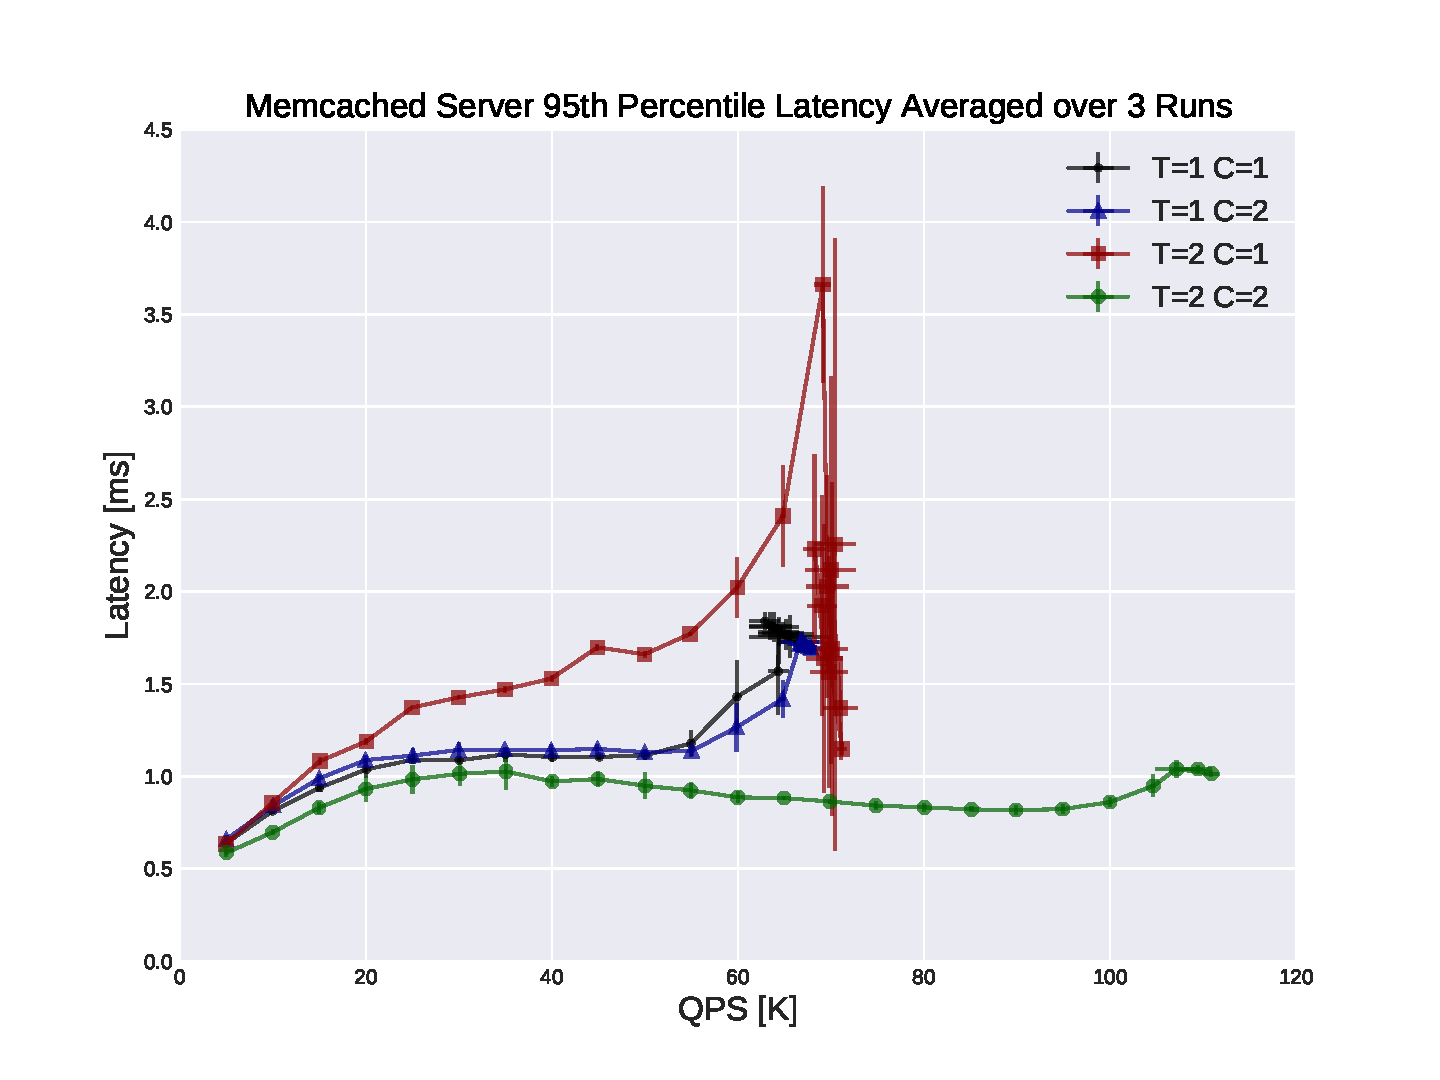
\includegraphics[width=0.9\textwidth]{p95.pdf}}
    \end{center}
    
    Performance with 2 threads and 2 cores (green line) is significantly better than other combinations. One core is not enough for memcached to support QPS larger than 60k-70k. If we use only 1 thread, giving it more cores doesn't help significantly. And if we use 2 thread with only 1 core, additional context switching between these 2 threads will damage the performance even further.

    \item \textbf{[8 points]} Now assume you need to support a memcached request load that ranges from 5K to 100K QPS while guaranteeing a 2ms 95th percentile latency SLO. \\
    

    
    a) To support the highest load in the trace (100K QPS) without violating the 2ms latency SLO, how many memcached threads ($T$) and CPU cores ($C$) will you need? i.e., what value of $T$ and $C$ would you select? \\
    
    \textbf{Solution:}
    
    I will use 2 threads and 2 cores. Other combinations do not support 100K QPS.\\
    
    b) Assume you can change the number of cores allocated to memcached dynamically as the QPS varies from 5K to 100K, but the number of threads is fixed when you launch the memcached job. How many memcached threads ($T$) do you propose to use to guarantee the 2ms 95th percentile latency SLO while the load varies between 5K to 100K QPS? i.e., what values of $T$ would you select? \\
    
    \textbf{Solution:}
    
    I will use 2 threads. We can support 100K QPS only when 2 threads are used.\\
    
    c) Run memcached with the number of threads $T$ that you proposed in b) above and measure performance with $C=1$ and $C=2$. Use the following \texttt{mcperf} command to sweep QPS from 5K to 100K:
    
    \begin{Verbatim}[fontsize=\small]
$ ./mcperf -s INTERNAL_MEMCACHED_IP --loadonly 
$ ./mcperf -s INTERNAL_MEMCACHED_IP -a INTERNAL_AGENT_IP  \
           --noload -T 16 -C 4 -D 4 -Q 1000 -c 4 -t 5 \ 
           --scan 5000:100000:5000
\end{Verbatim}

    Measure the CPU utilization on the memcached server at each 5-second load time step.
    
    Plot the performance of memcached using 1-core ($C=1$) and using 2 cores ($C=2$) in \textbf{two separate graphs}, for $C=1$ and $C=2$,  respectively. In each graph, plot QPS on the x-axis, ranging from 5K to 100K. In each graph, use two y-axes. Plot the 95th percentile latency on the left y-axis. Draw a dotted horizontal line at the 2ms latency SLO. Plot the CPU utilization (ranging from 0\% to 100\% for $C=1$ or 200\% for $C=2$) on the right y-axis. For simplicity, we do not require error bars for these plots. 
    %Plot a scatter plot with CPU utilization on the x-axis and 95th percentile latency on the y-axis. Your plot should have two lines in your plot: one with a 1-core memcached server ($C=1$) and one with a 2-core memcached server ($C=2$). For simplicity, we do not require error bars for this plot. \todo{Decide which kind of plot is best. QPS too?}
    
    \textbf{Solution:}
    \begin{center}
    {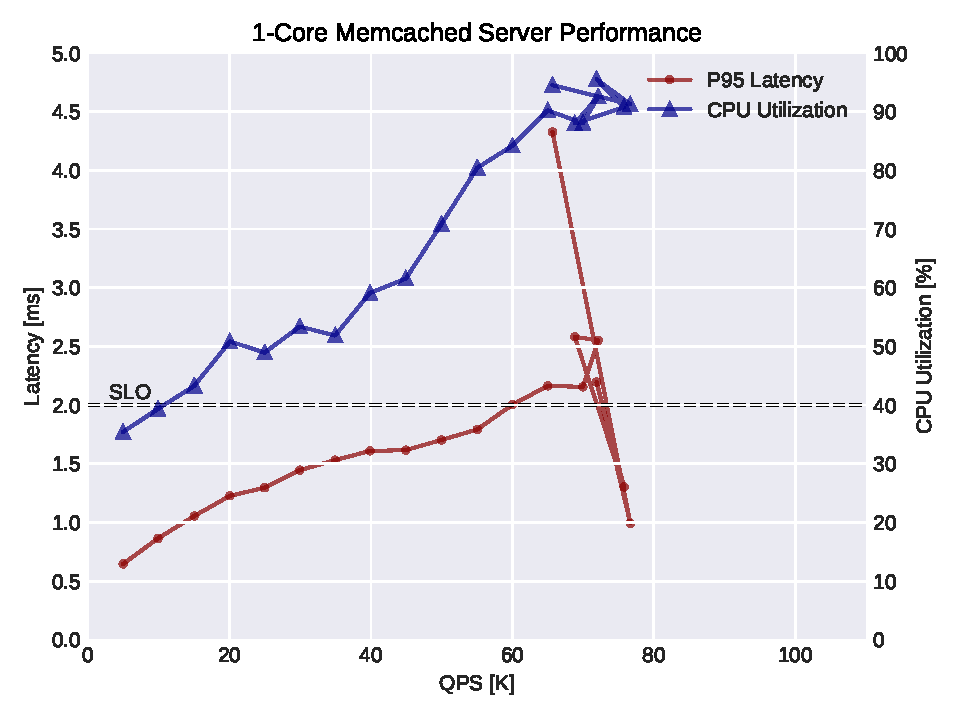
\includegraphics[width=0.9\textwidth]{c1.pdf}}
    \end{center}
    \begin{center}
    {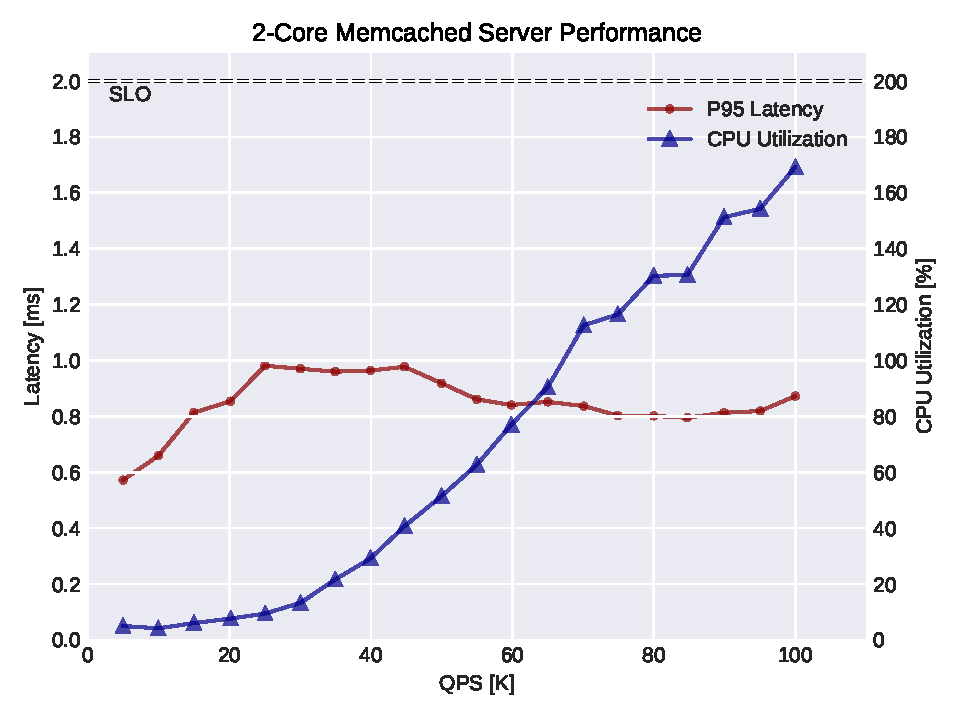
\includegraphics[width=0.9\textwidth]{c2.pdf}}
    \end{center}
    
    \item \textbf{[15 points]} You are now given a dynamic load trace for memcached, which varies QPS randomly between 5K and 100K in 10 second time intervals. Use the following command to run this trace: 
        \begin{Verbatim}[fontsize=\small]
$ ./mcperf -s INTERNAL_MEMCACHED_IP --loadonly 
$ ./mcperf -s INTERNAL_MEMCACHED_IP -a INTERNAL_AGENT_IP \ 
           --noload -T 16 -C 4 -D 4 -Q 1000 -c 4 -t 1800 \ 
           --qps_interval 10 --qps_min 5000 --qps_max 100000
\end{Verbatim}
    
    Note that you can also specify a random seed in this command using the \texttt{--qps\_seed} flag. \\
    
    Design and implement a controller to schedule memcached and the PARSEC benchmarks on the 4-core VM. The goal of your scheduling policy is to successfully complete all PARSEC jobs as soon as possible without violating the 2ms 95th percentile latency for memcached. \textbf{Your controller should not assume prior knowledge of the dynamic load trace. You should design your policy to work well regardless of the random seed.} Also make sure to check that all the PARSEC jobs complete successfully and do not crash. Note that PARSEC jobs may fail if given insufficient resources. \\
    
    Describe how you designed and implemented your scheduling policy. Include the source code of your controller in the zip file you submit. To describe your scheduling policy, you should at minimum answer the following questions. For each, also \textbf{explain why}:
    \begin{itemize}
        \item How do you decide how many cores to dynamically assign to memcached? 
        \item How do you decide how many cores to assign each PARSEC job? 
        \item How many threads do you use for each of the PARSEC apps? 
        \item Which jobs run concurrently / are collocated and on which cores? 
        \item In which order did you run the PARSEC apps? 
        \item How does your policy differ from the policy in Part 3? 
        \item How did you implement your policy? e.g., docker cpu-set updates, taskset updates for memcached, pausing/unpausing containers, etc.
    \end{itemize}
    
    \textbf{Solution:}

Based on question 2(b), we decide to run memcached using 2 threads. If CPU usage of memcached is higher than 90\%, we assign 2 cores to it. If the usage drops below 90\%, we assign only 1 core to it. We choose 90\% as the threshold because, according to the graphs of question 2(c), it needs to change to 2 cores when the QPS is greater than 60K, and the corresponding CPU usage for QPS greater than 60K is above 90\%.

The VM has 4 cores in total. When memcached uses 2 cores, we use the remaining 2 cores to run PARSEC jobs. When memcached uses only 1 core, we use the remaining 3 cores to run PARSEC jobs. We have observed that the interference is very high when 2 PARSEC jobs are running at the same time. It costs more time to run in parallel than to run sequentially. So, our basic idea is to run the jobs sequentially with 3 threads for each job. However, fft does not support 3 threads. We also find that some jobs are not fully parallelizable, which has a long preprocessing or postprocessing stage when they can only run with 1 thread. As an optimization, we run fft in 2 threads and use pause/unpause function to let fft run only when other jobs are in single thread stage. In this way, we can fully utilize the CPU cores by ensuring there are 3  threads running nearly all the times. The 3 threads are always running in the same CPU set (2 or 3 cores). We do not assign a dedicated core to a specific job, so that we have more flexibility to deal with different random seeds.

    The picture below depicts our schedule policy. For simplicity, the time is not drawn proportional to real time. Core 0 and 1 are assigned to PARSEC jobs, core 3 is assigned to memcached, and core 2 is dynamically assigned. We run dedup, blackscholes, canneal, ferret, and freqmine sequentially. And we also let fft run in the single thread stages of dedup, blackscholes, and canneal. We choose this order because the first 3 jobs have a longer single thread stage which can allow fft to finish, while on the other hand, ferret and freqmine almost do not have a single thread stage.

\begin{center}
  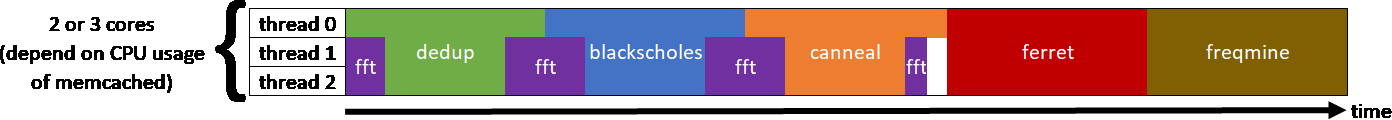
\includegraphics[width=0.9\textwidth]{part4q3.png}  
\end{center}


The main difference to part 3 is the core allocation is dynamically adjusted to adapt the changing QPS of memcached. Moreover, because we only use one VM in part 4, the jobs are mainly running in sequence instead of in parallel.

We write our scheduler in python. We check the status and perform scheduling operations every 0.5 second, which is small enough compared to the 10 seconds interval. We use Docker Python SDK for PARSEC jobs (start/remove jobs, update CPU sets, pause/unpause jobs, collect logs, etc.). We execute taskset command to change CPU sets for memcached. We execute top command to get precise CPU usage of memcached and pid of PARSEC jobs. We read /proc/\textless pid\textgreater/status files to get the current number of threads of PARSEC jobs.

    \item \textbf{[23 points]} Run the following \texttt{mcperf} memcached dynamic load trace: 
    
            \begin{Verbatim}[fontsize=\small]
$ ./mcperf -s INTERNAL_MEMCACHED_IP --loadonly 
$ ./mcperf -s INTERNAL_MEMCACHED_IP -a INTERNAL_AGENT_IP \ 
           --noload -T 16 -C 4 -D 4 -Q 1000 -c 4 -t 1800 \ 
           --qps_interval 10 --qps_min 5000 --qps_max 100000 \ 
           --qps_seed 42
\end{Verbatim}
    
    
    Measure memcached and PARSEC performance when using your scheduling policy to launch workloads and dynamically adjust container resource allocations. Run this workflow 3 separate times. For each run, measure the execution time of each PARSEC job, as well as the latency outputs of memcached. For each PARSEC application, compute the mean and standard deviation of the execution time across three runs. Also compute the mean and standard deviation of the total time to complete all jobs. Fill in the table below.  Also compute the SLO violation ratio for memcached for each of the three runs; the number of datapoints with 95th percentile latency \textgreater \ 2ms, as a fraction of the total number of datapoints.  \\
    
    \textbf{Solution:}
    
    \begin{table}[h]
        \centering
        \begin{tabular}{ |c|c|c|c|c|} 
        \hline
        job name & mean time [s] & std [s] \\
        \hhline{|=|=|=|}
        dedup         & 45.8 & 1.16 \\ \hline
        blackscholes  & 155.7 & 3.11 \\ \hline
        ferret        & 586.5 & 3.13 \\ \hline
        freqmine      & 278.1 & 2.07 \\ \hline
        canneal       & 295.2 & 1.74 \\ \hline
        fft           & 149.9 & 3.78 \\ \hline
        total time    & 1363.9 & 11.04 \\ \hline
        \end{tabular}
    \end{table}

    SLO violation ratio: \\
    Run 1: 0 / 138 = 0 \% \\
    Run 2: 0 / 137 = 0 \% \\
    Run 3: 2 / 136 = 1.5 \% \\

   Include six plots -- two plots for each of the three runs -- with the following information. Label the plots as 1A, 1B, 2A, 2B, 3A, and 3B where the number indicates the run and the letter indicates the type of plot (A or B), which we describe below. In all plots, time will be on the x-axis and you should annotate the x-axis to indicate which PARSEC benchmark starts executing at which time. If you pause/unpause any workloads as part of your policy, you should also indicate the timestamps at which jobs are paused and unpaused. All the plots will have have two y-axes. The right y-axis will be QPS. For Plots A, the left y-axis will be the 95th percentile latency. For Plots B, the left y-axis will be the number of CPU cores that your controller allocates to memcached. 

    \textbf{Solution:}
    
    The horizontal bar below the graph indicates the time range when a PARSEC job is running.
    
    \begin{center}
    {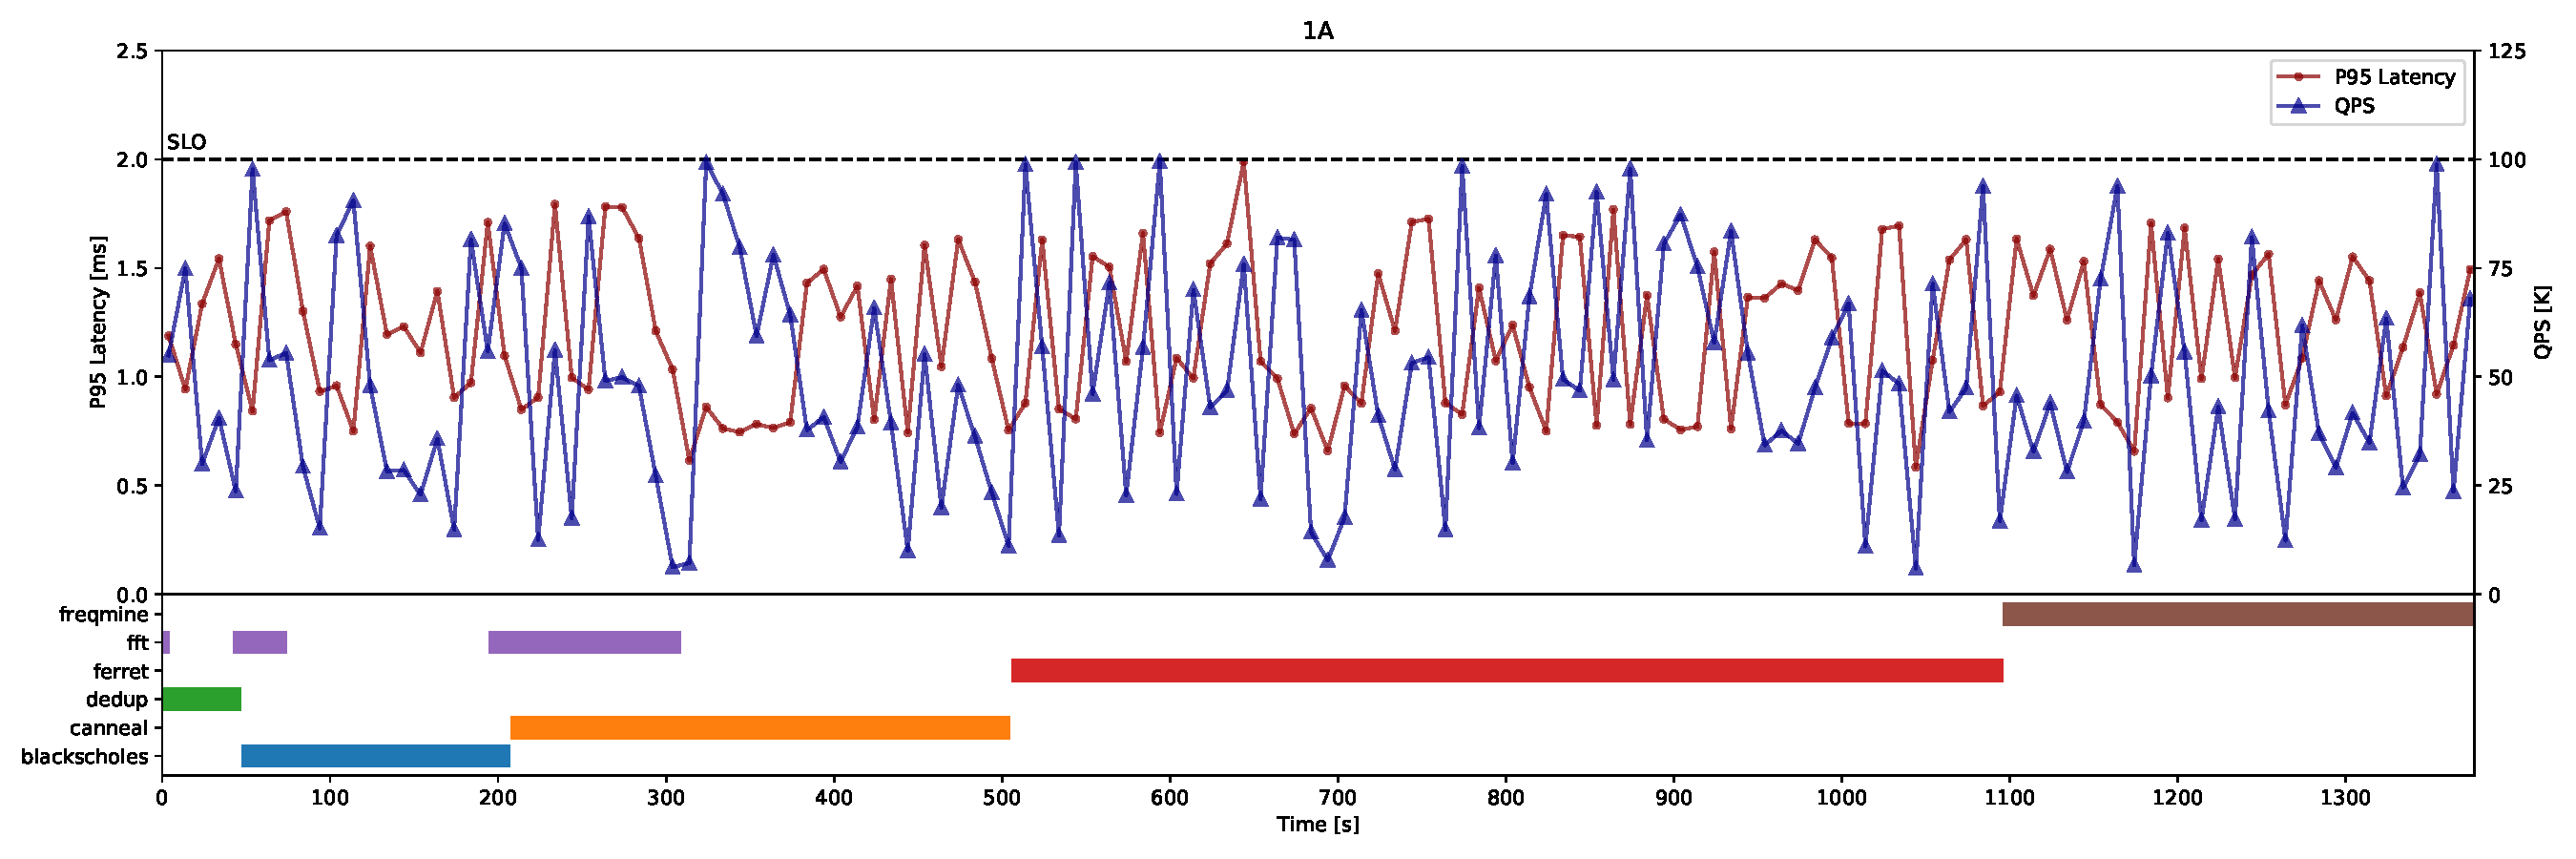
\includegraphics[width=0.9\textwidth]{plot10/1A.pdf}}
    \end{center}
    \begin{center}
    {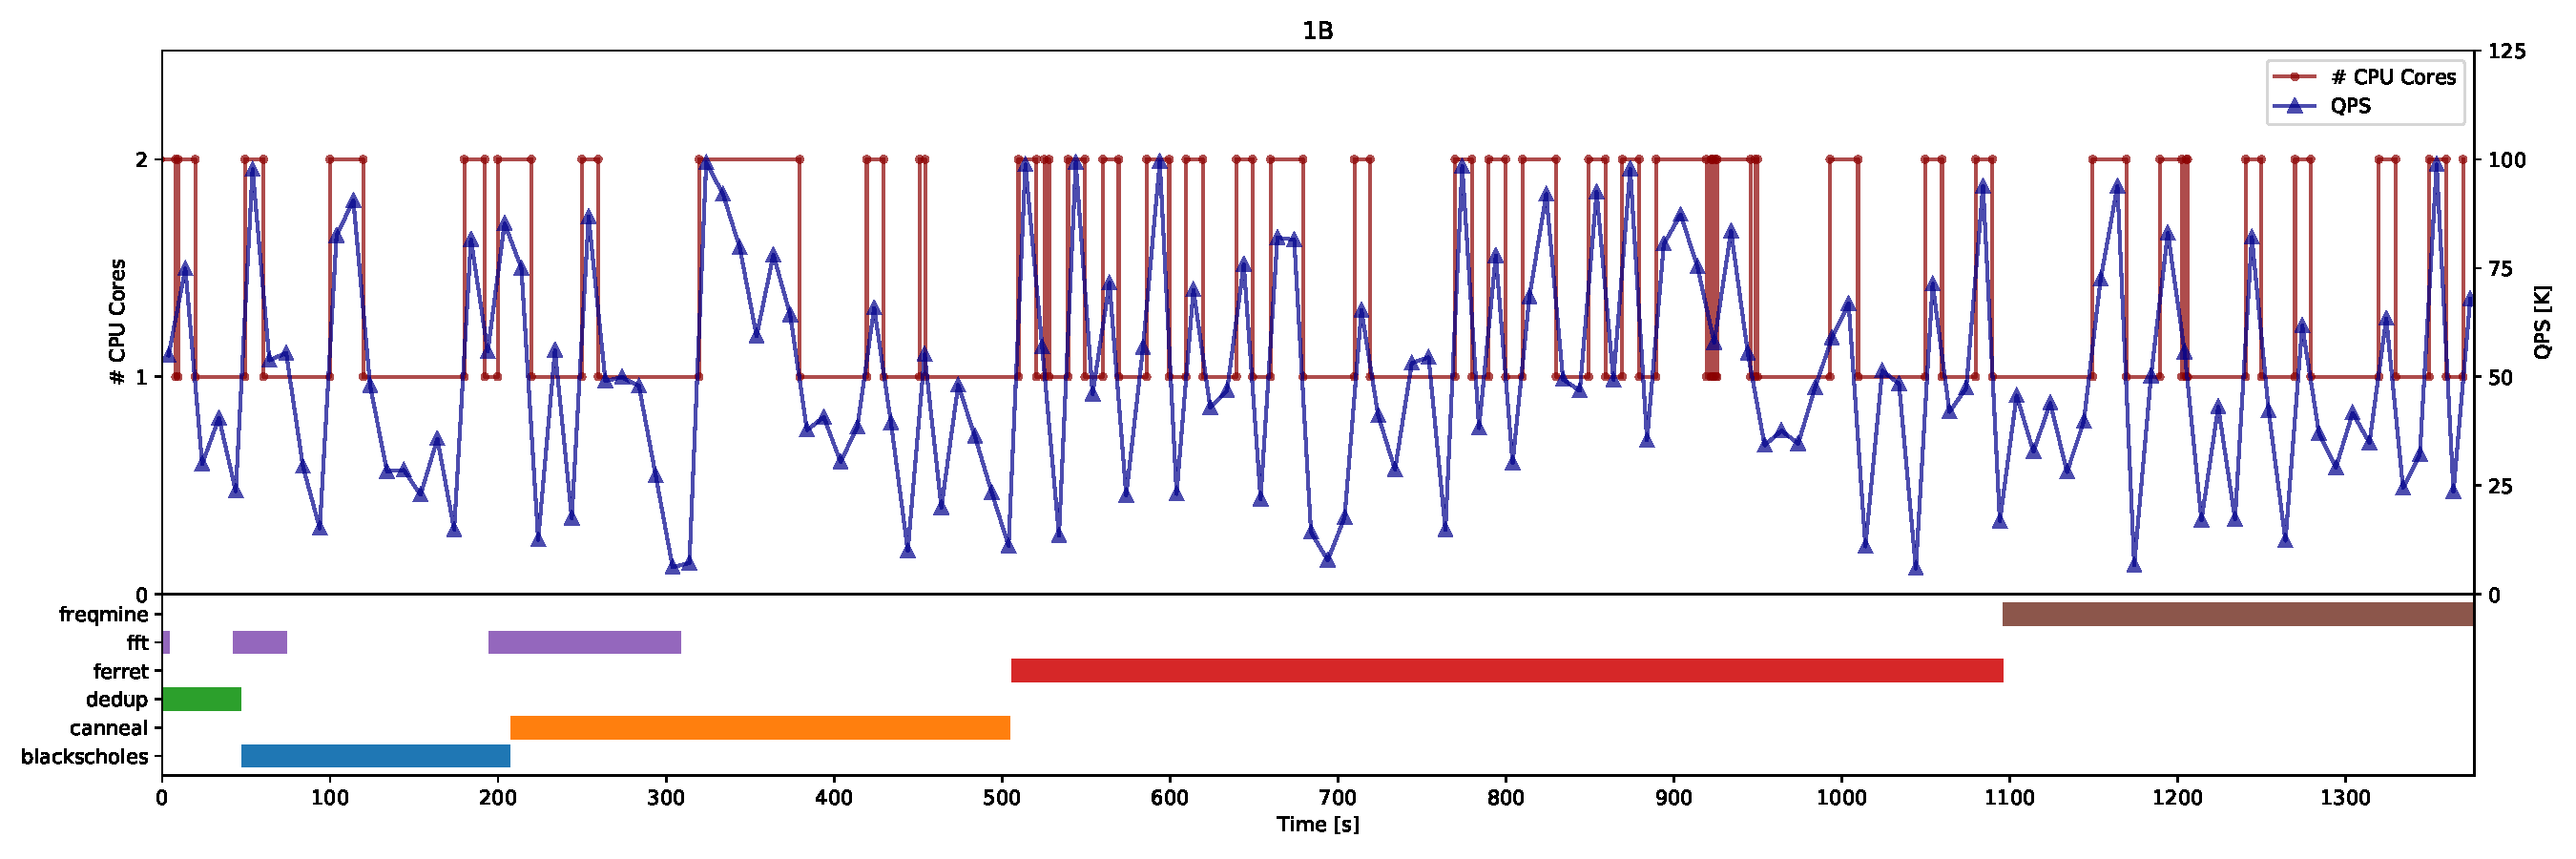
\includegraphics[width=0.9\textwidth]{plot10/1B.pdf}}
    \end{center}
    \begin{center}
    {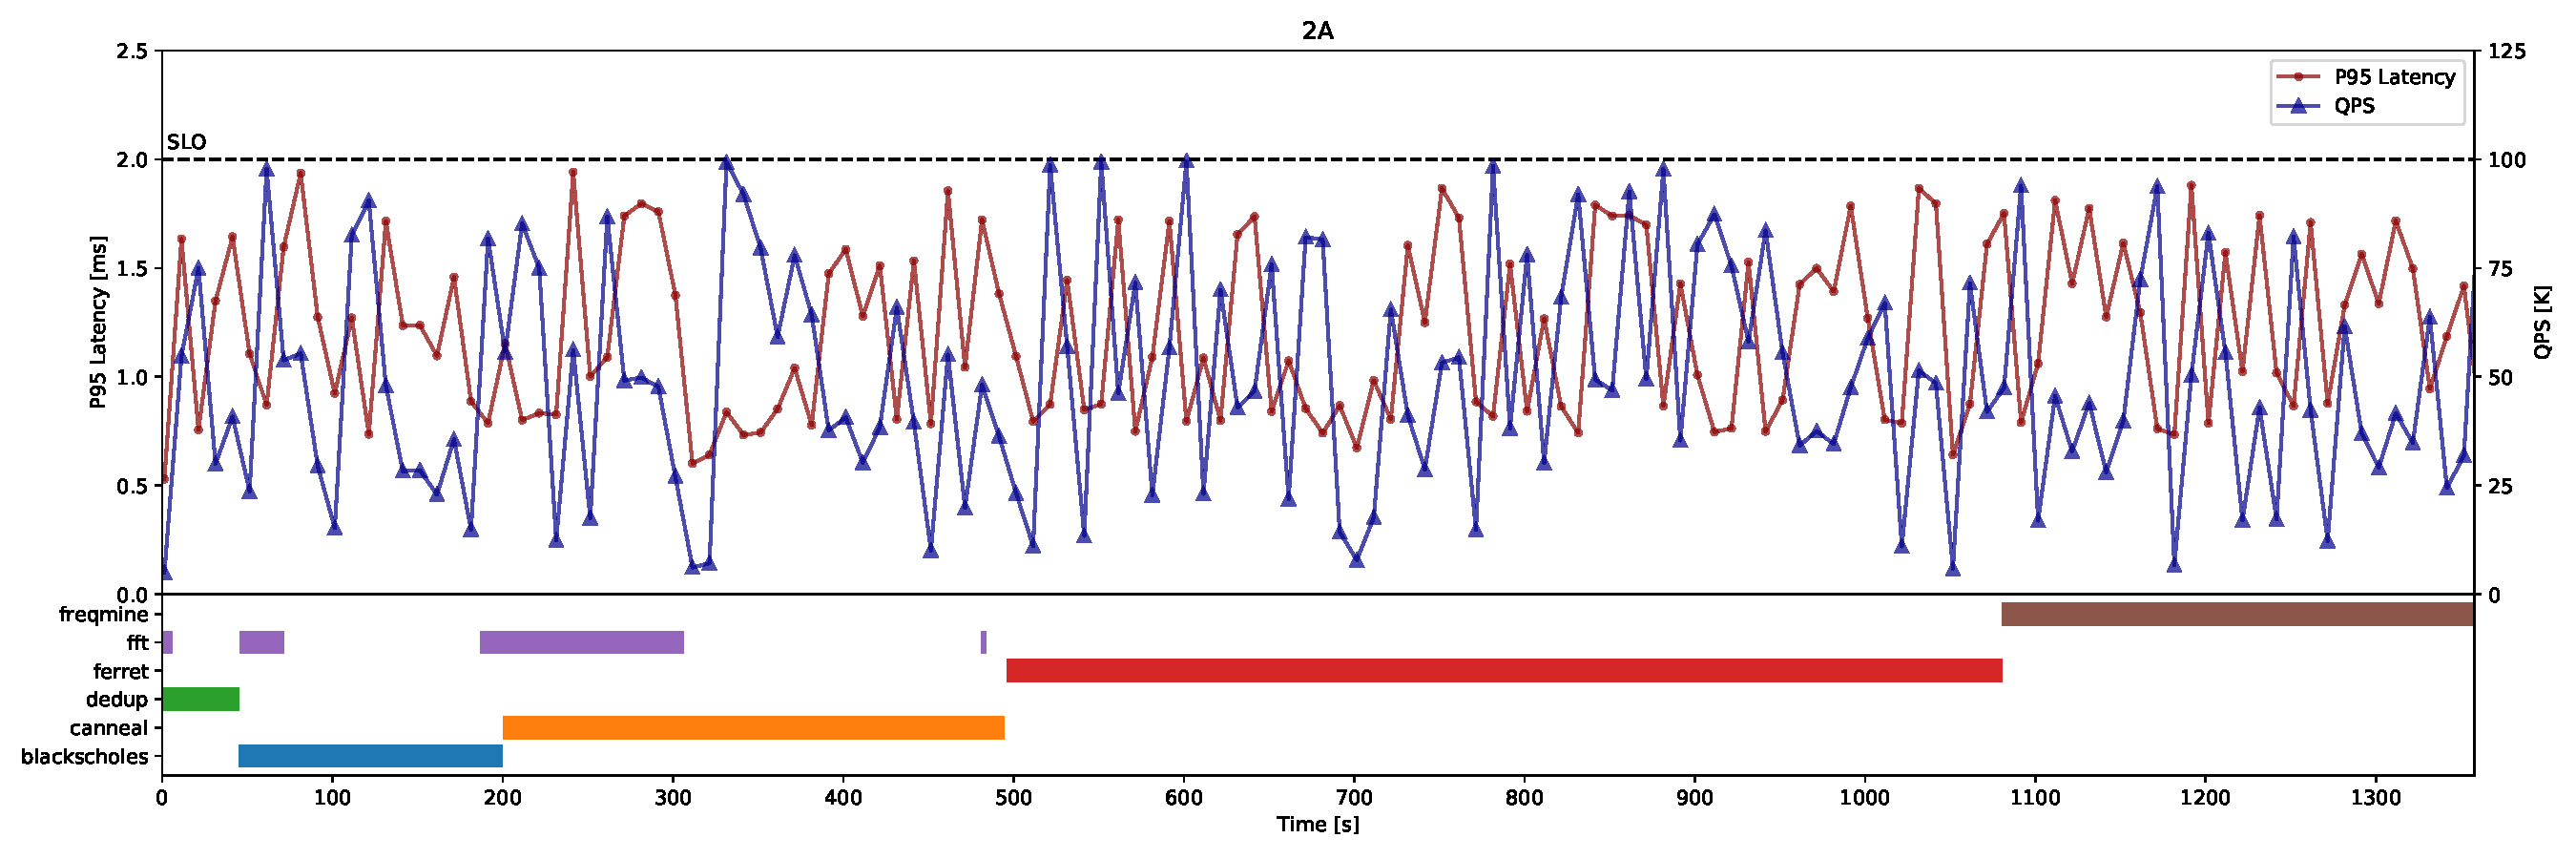
\includegraphics[width=0.9\textwidth]{plot10/2A.pdf}}
    \end{center}
    \begin{center}
    {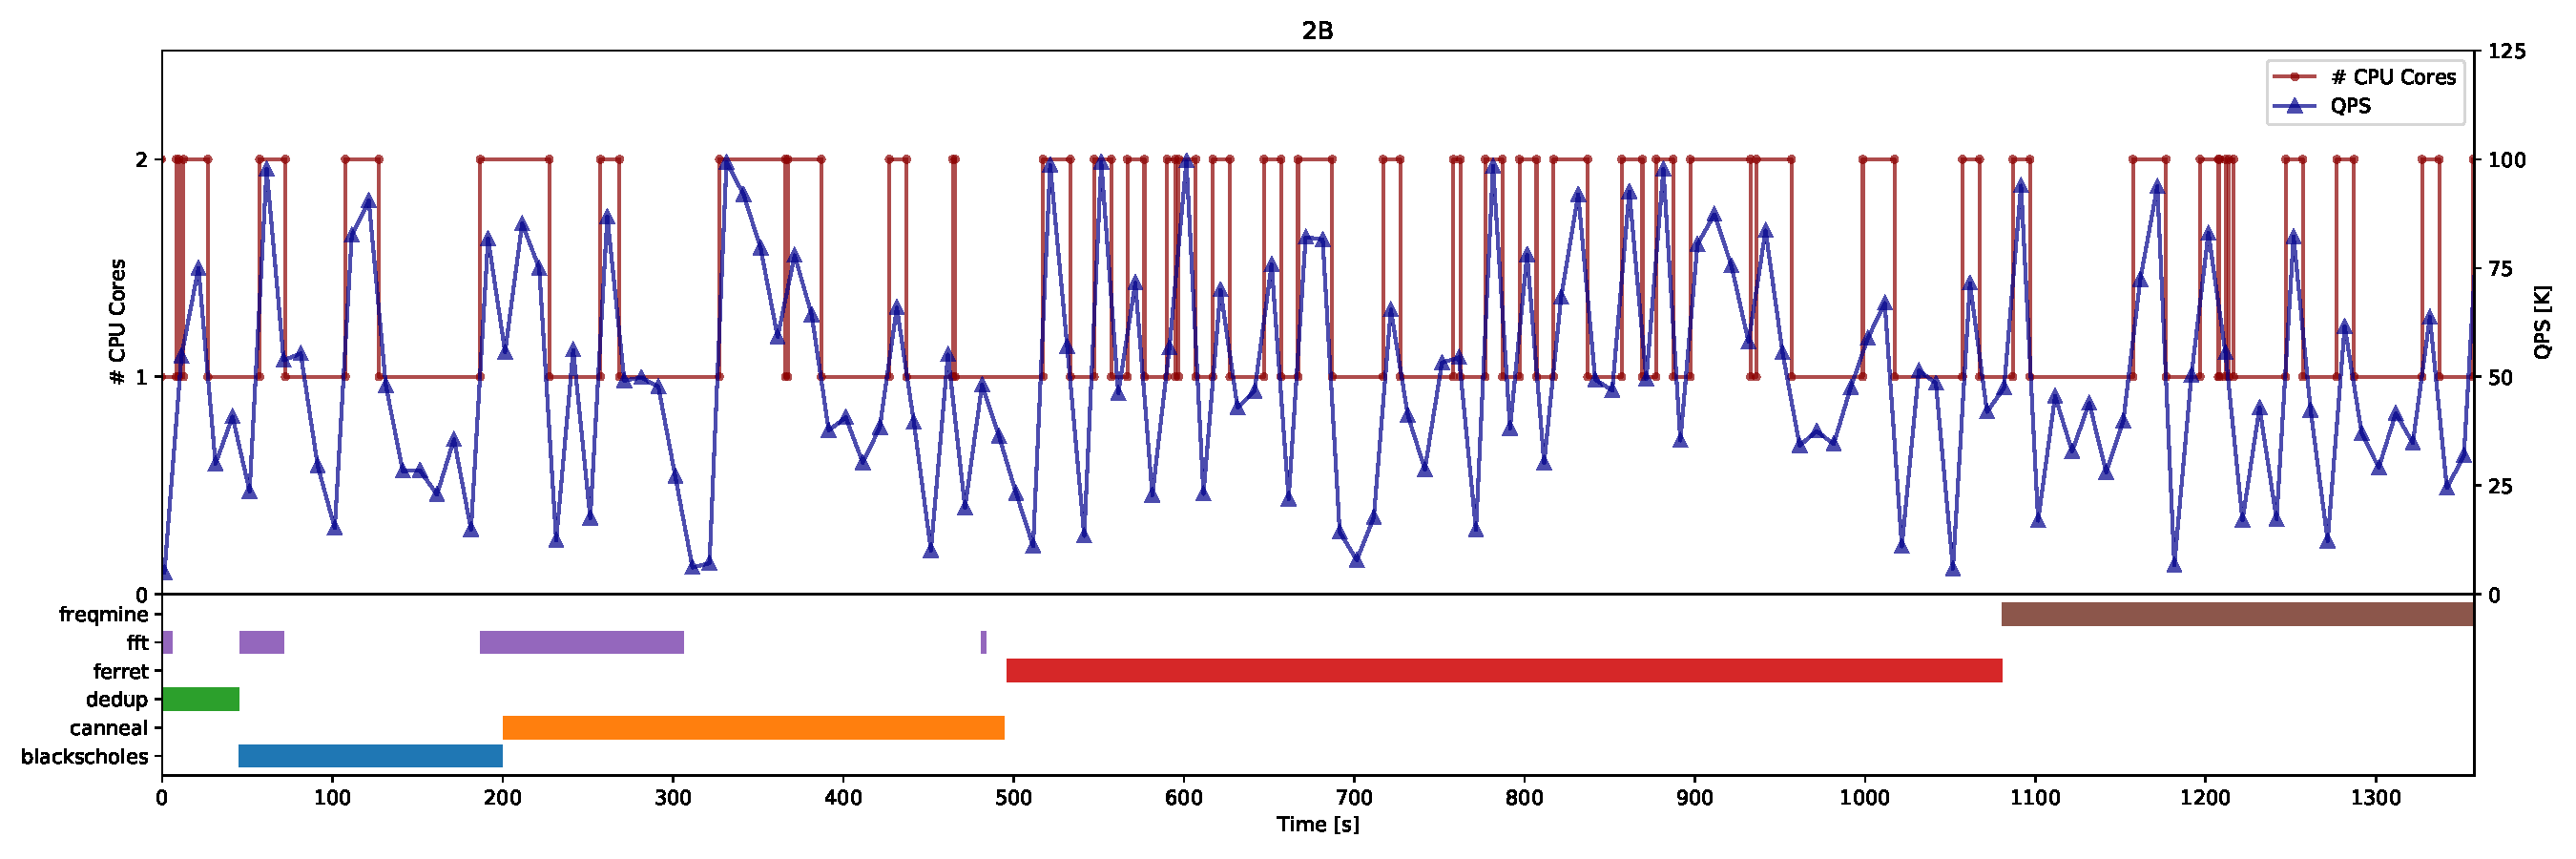
\includegraphics[width=0.9\textwidth]{plot10/2B.pdf}}
    \end{center}
    \begin{center}
    {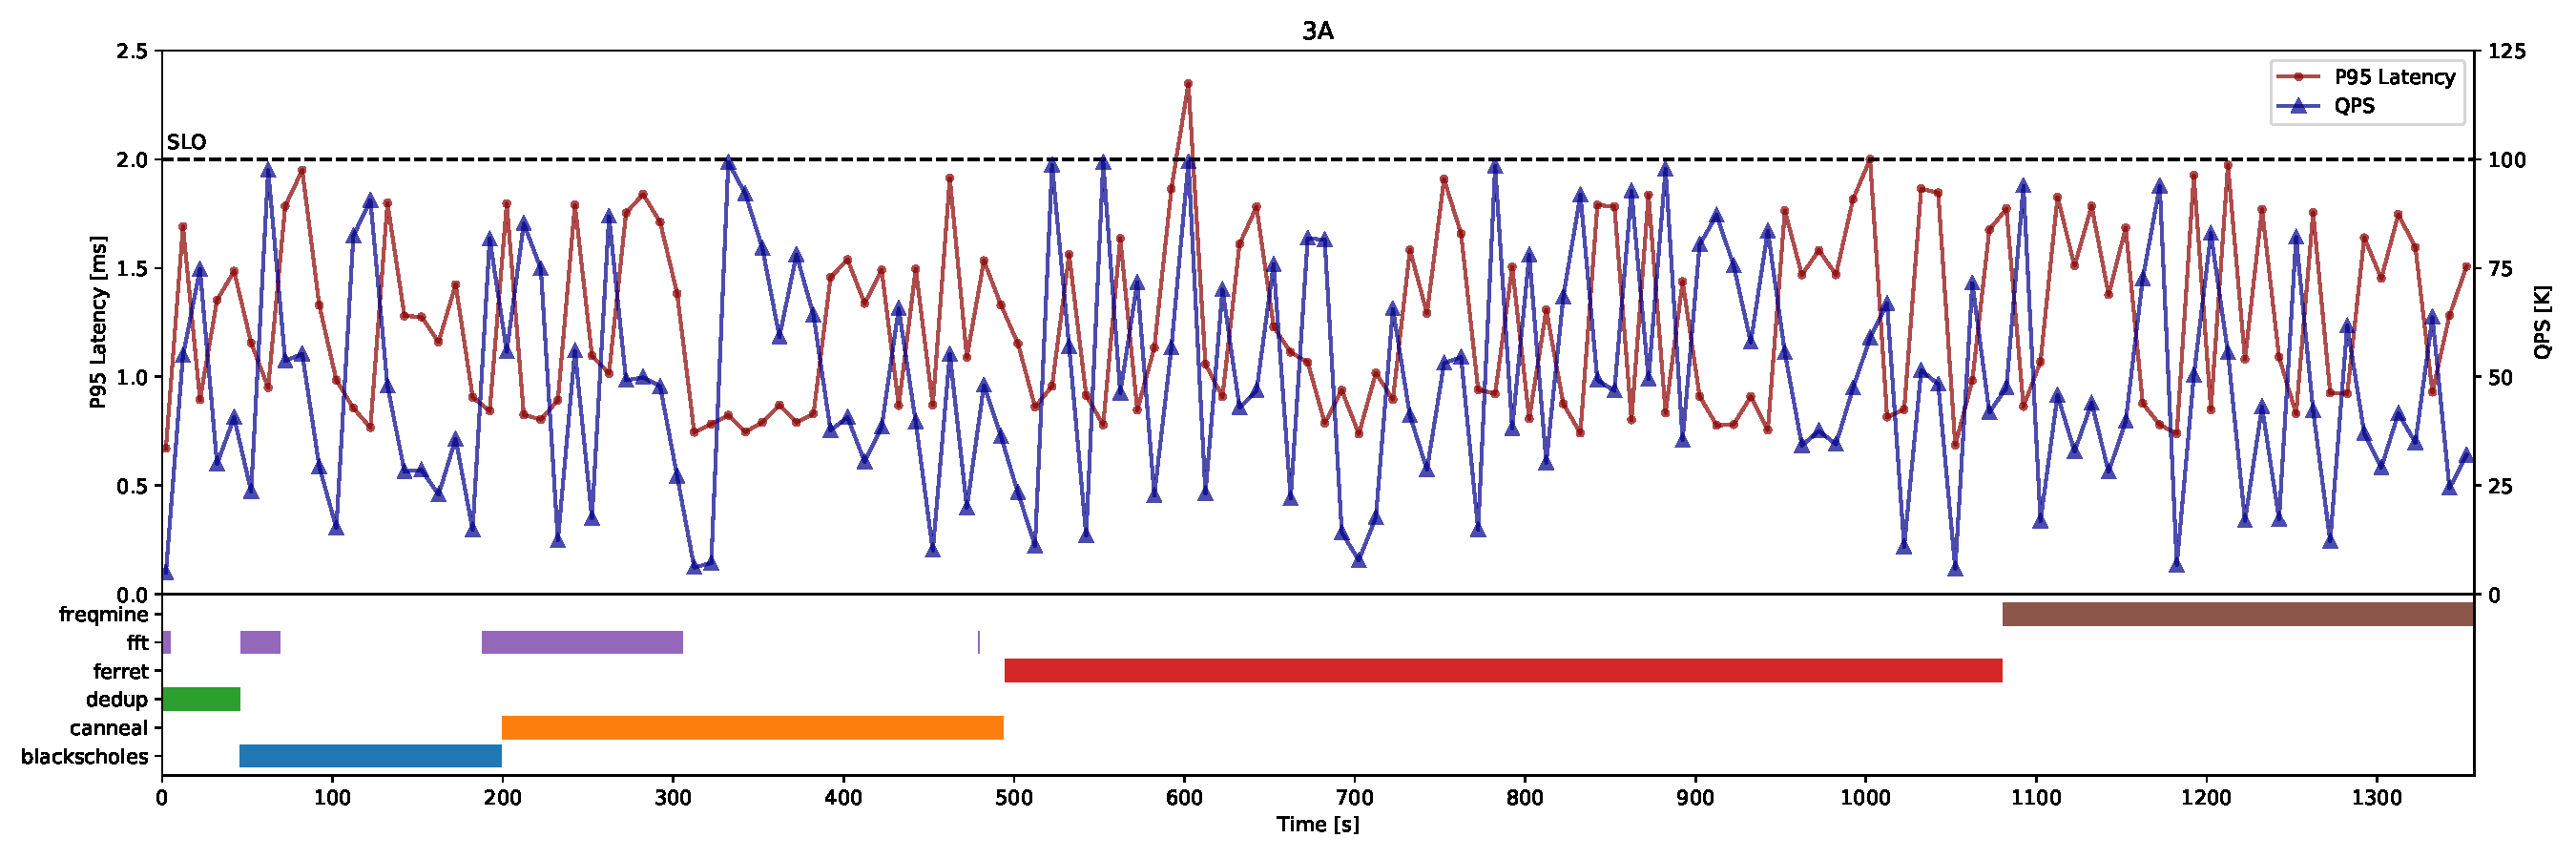
\includegraphics[width=0.9\textwidth]{plot10/3A.pdf}}
    \end{center}
    \begin{center}
    {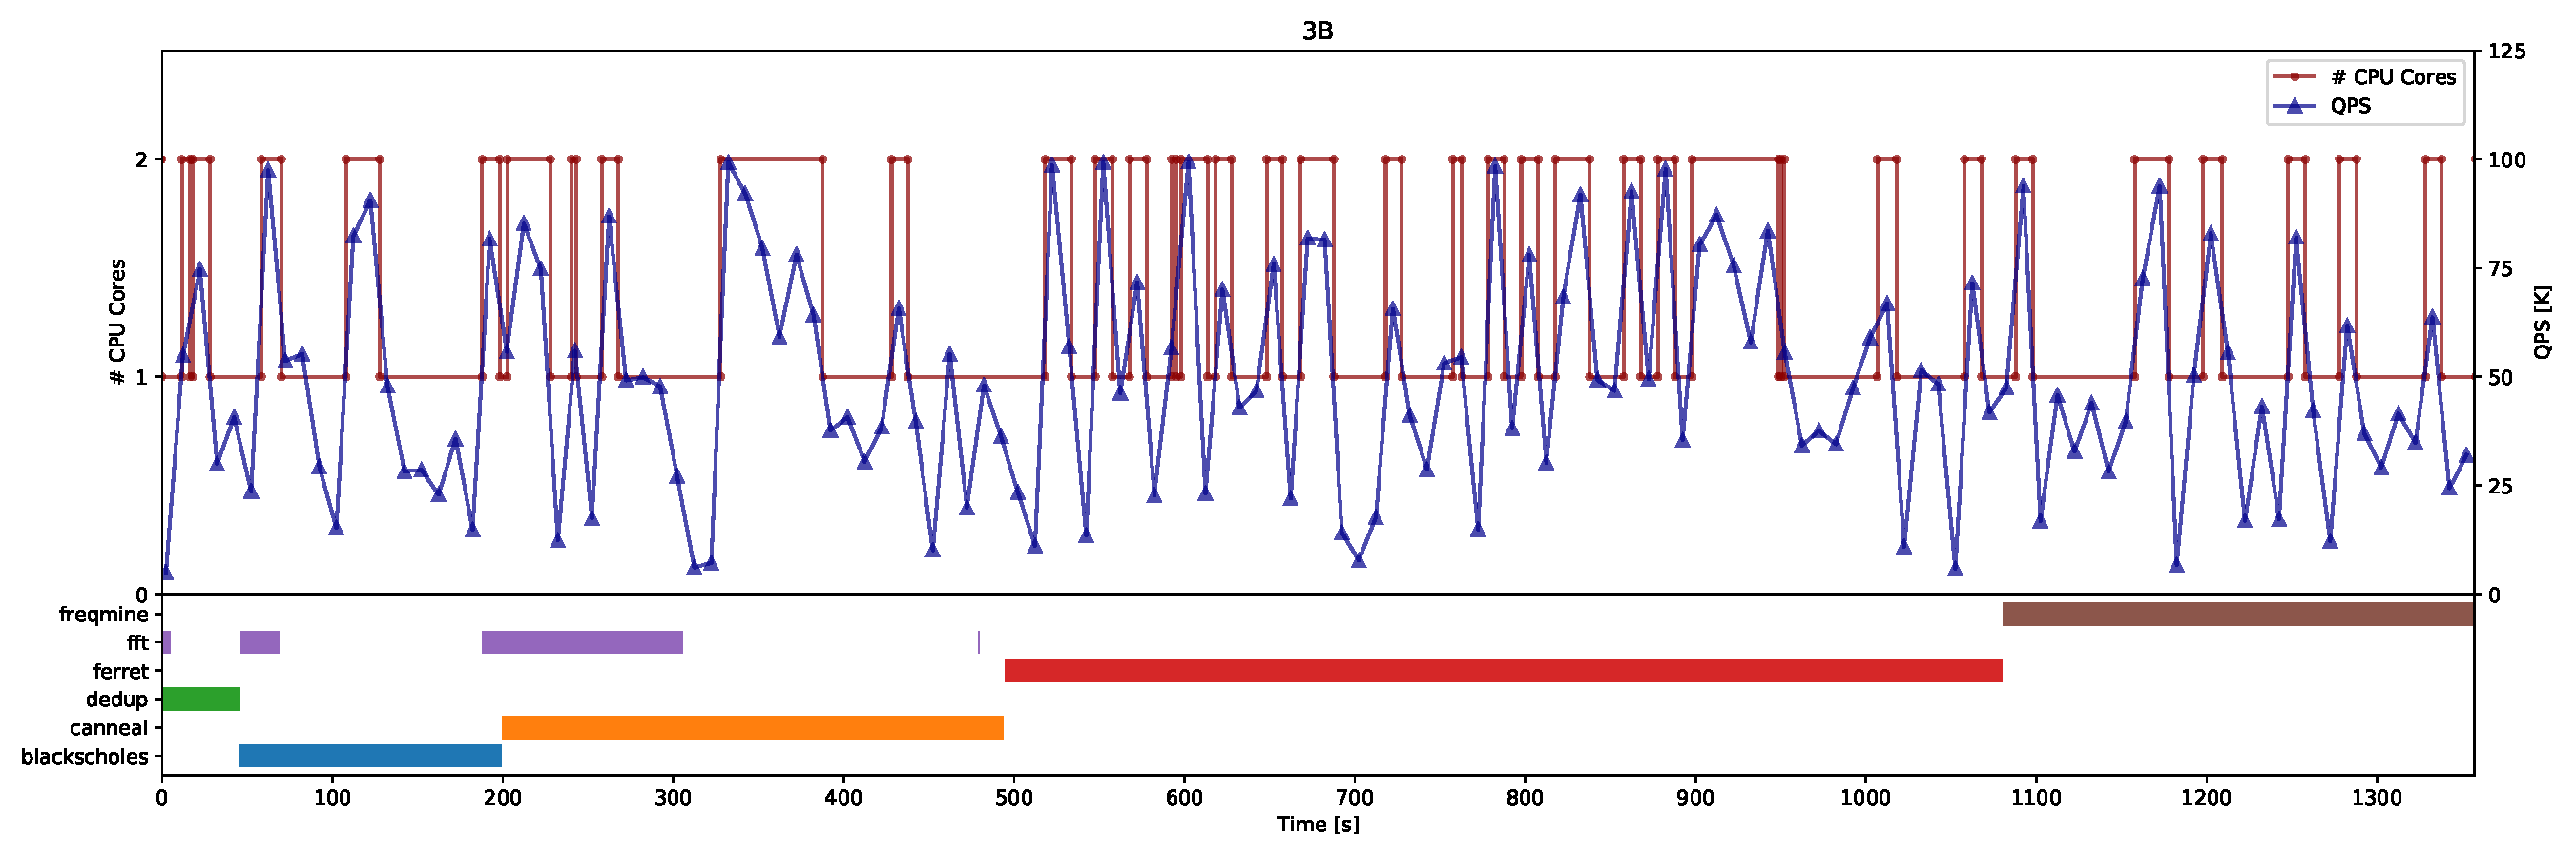
\includegraphics[width=0.9\textwidth]{plot10/3B.pdf}}
    \end{center}

    \item \textbf{[20 points]} Repeat Part 4 Question 4 with a modified \texttt{mcperf} dynamic load trace with a 5 second time interval (\texttt{qps\_interval}) instead of 10 second time interval. Use the following command: 
    
                \begin{Verbatim}[fontsize=\small]
$ ./mcperf -s INTERNAL_MEMCACHED_IP --loadonly 
$ ./mcperf -s INTERNAL_MEMCACHED_IP -a INTERNAL_AGENT_IP \ 
           --noload -T 16 -C 4 -D 4 -Q 1000 -c 4 -t 1800 \ 
           --qps_interval 5 --qps_min 5000 --qps_max 100000 \ 
           --qps_seed 42
\end{Verbatim}
    
    You do not need to include the plots or table from Question 4 for the 5-second interval. Instead, summarize in 2-3 sentences how your policy performs with the smaller time interval (i.e., higher load variability) compared to the original load trace in Question 4. What is the SLO violation ratio for memcached (i.e., the number of datapoints with 95th percentile latency \textgreater \ 2ms, as a fraction of the total number of datapoints)  with the 5-second time interval trace? \\
    
    \textbf{Solution:}

    The average total running time is 1396.8 seconds, slightly larger than that of the 10-second interval. The CPU core allocation is changed more frequently to adapt the faster changing QPS load, which may cause some overhead.
    
    The SLO violation ratio becomes larger. With more variations in QPS, there are more chances that the scheduler may not be able to react immediately when the QPS suddenly increase, and so SLO is violated more often.
    
    SLO violation ratio: \\
    Run 1: 1 / 277 = 0.4 \% \\
    Run 2: 5 / 281 = 1.8 \% \\
    Run 3: 1 / 283 = 0.4 \%  \\
    
    What is the smallest \texttt{qps\_interval} you can use in the load trace that allows your controller to respond fast enough to keep the memcached SLO violation ratio under 3\%? Use this \texttt{qps\_interval} in the command above and collect results for three runs. Include the same types of plots (1A, 1B, 2A, 2B, 3A, 3B) and table as in Question 4. 
    
    \textbf{Solution:}
    
    The smallest \texttt{qps\_interval} is 2 seconds.

    \begin{table}[h]
        \centering
        \begin{tabular}{ |c|c|c|c|c|} 
        \hline
        job name & mean time [s] & std [s] \\
        \hhline{|=|=|=|}
        dedup         & 43.7 & 3.68 \\  \hline
        blackscholes  & 164.1 & 2.85 \\  \hline
        ferret        & 593.8 & 1.36 \\  \hline
        freqmine      & 305.2 & 5.12 \\  \hline
        canneal       & 304.8 & 2.88 \\  \hline
        fft           & 147.4 & 3.87 \\  \hline
        total time    & 1414.0 & 6.21 \\ \hline
        \end{tabular}
    \end{table}
    
    SLO violation ratio: \\
    Run 1: 5 / 707 = 0.7 \% \\
    Run 2: 15 / 711 = 2.1 \% \\
    Run 3: 4 / 705 = 0.6 \% \\
    
    \begin{center}
    {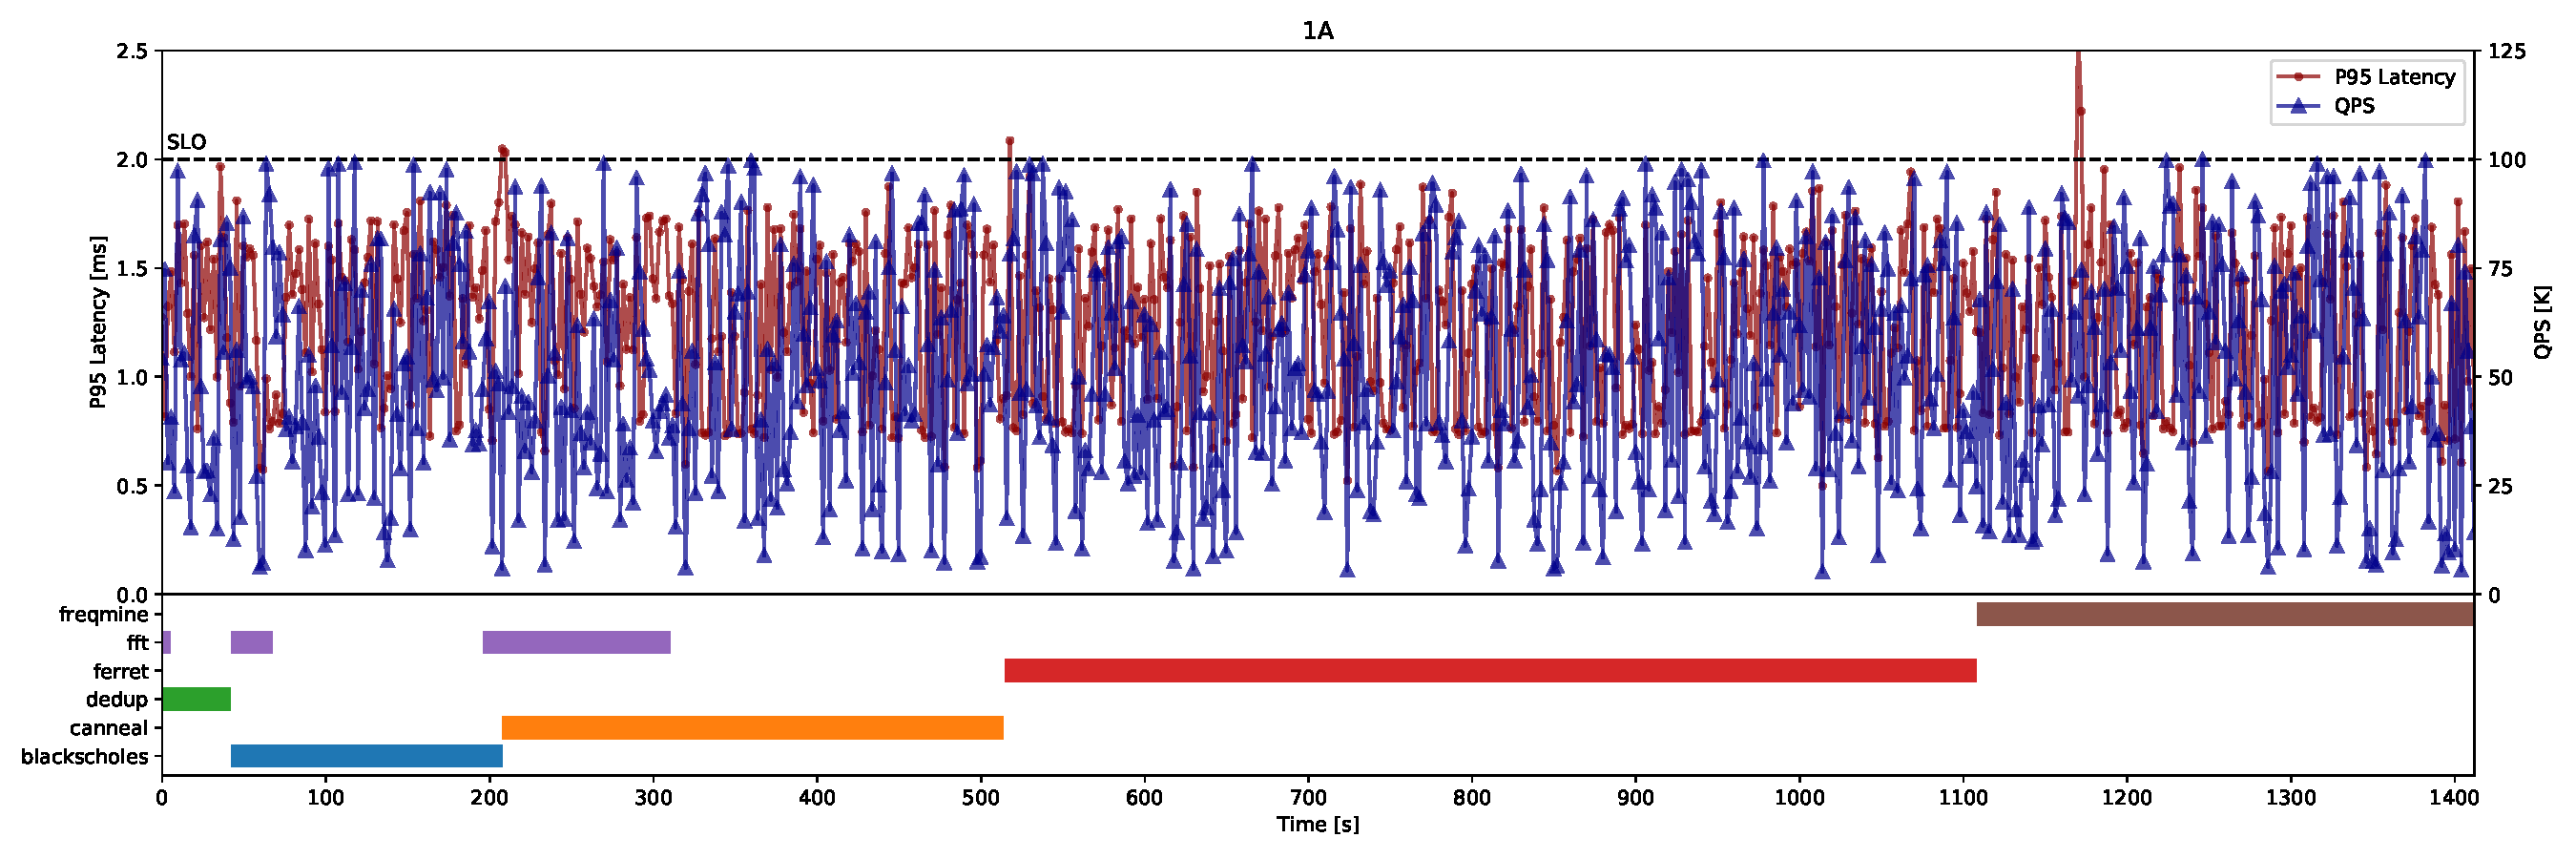
\includegraphics[width=0.9\textwidth]{plot2/1A.pdf}}
    \end{center}
    \begin{center}
    {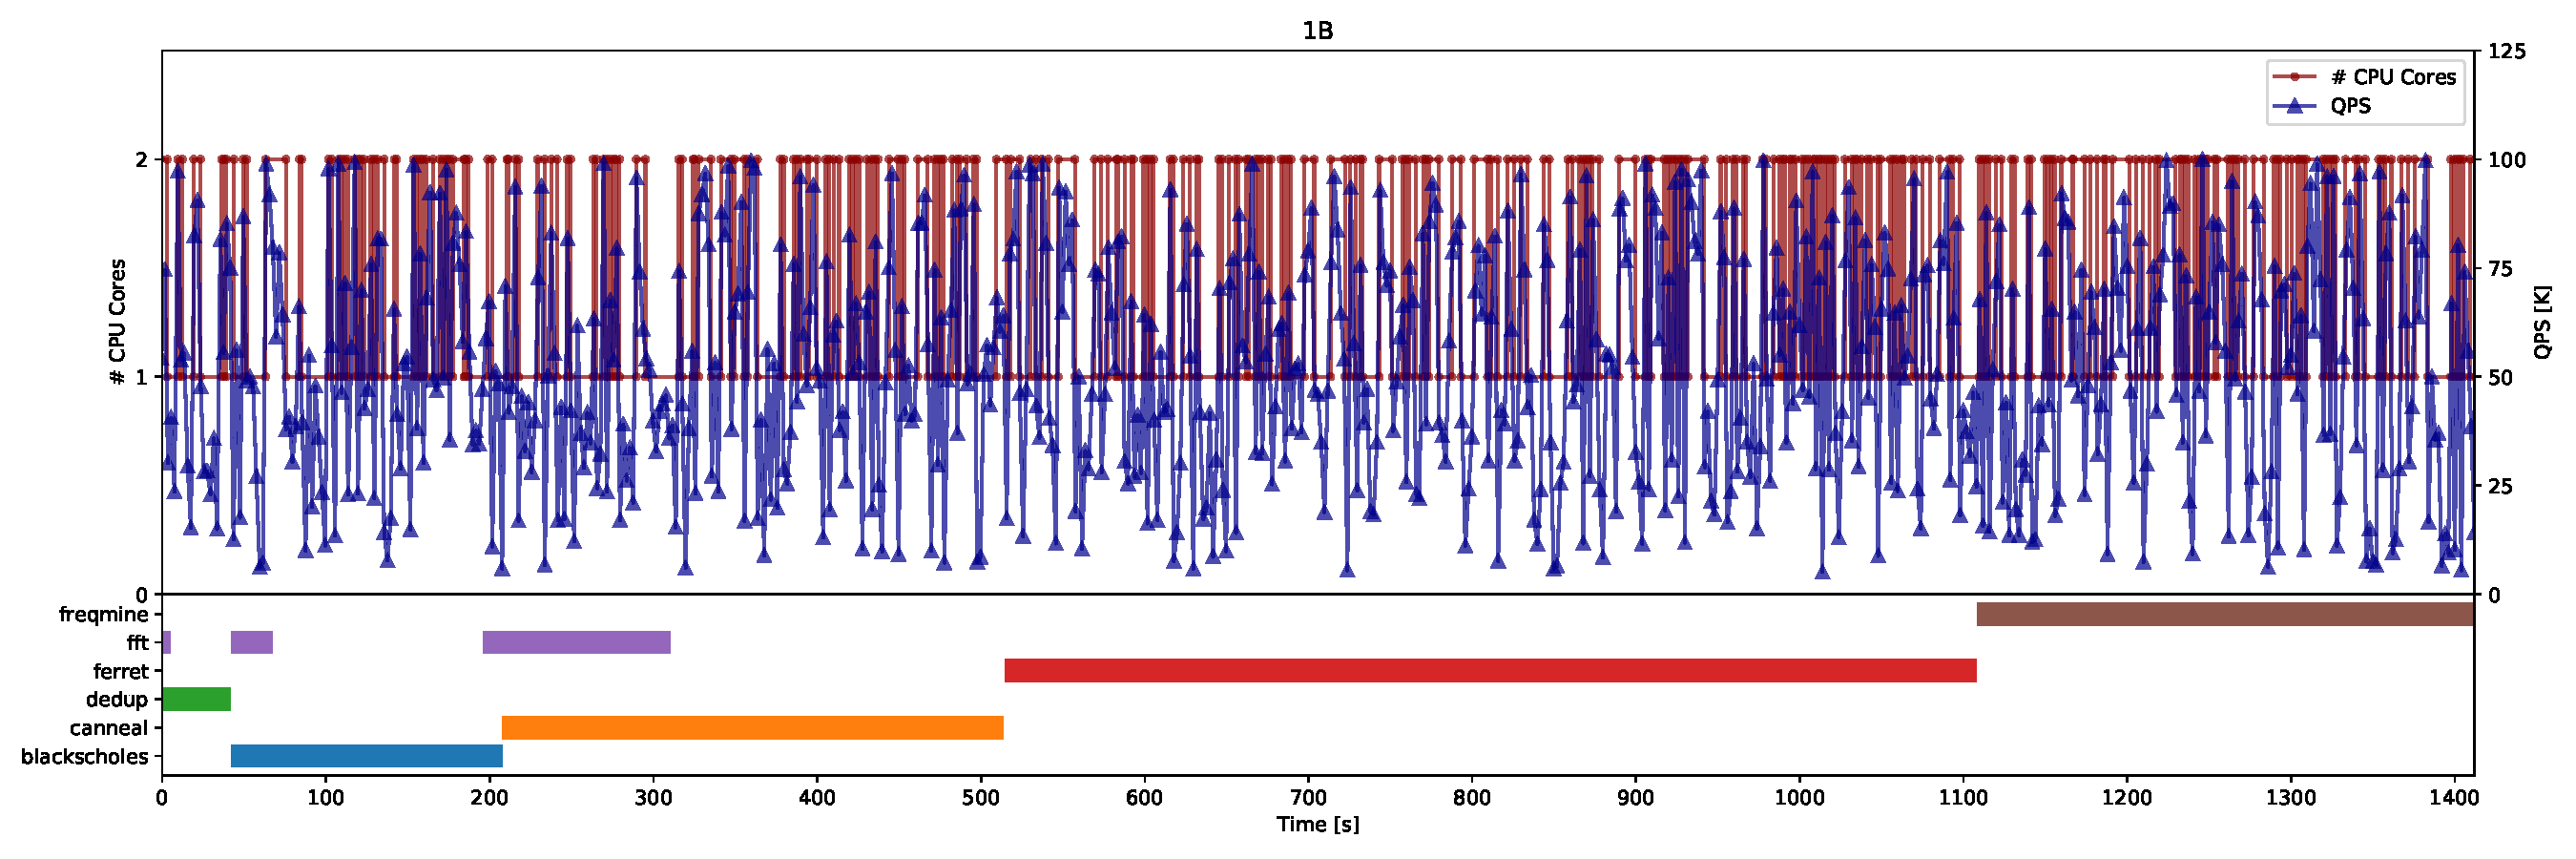
\includegraphics[width=0.9\textwidth]{plot2/1B.pdf}}
    \end{center}
    \begin{center}
    {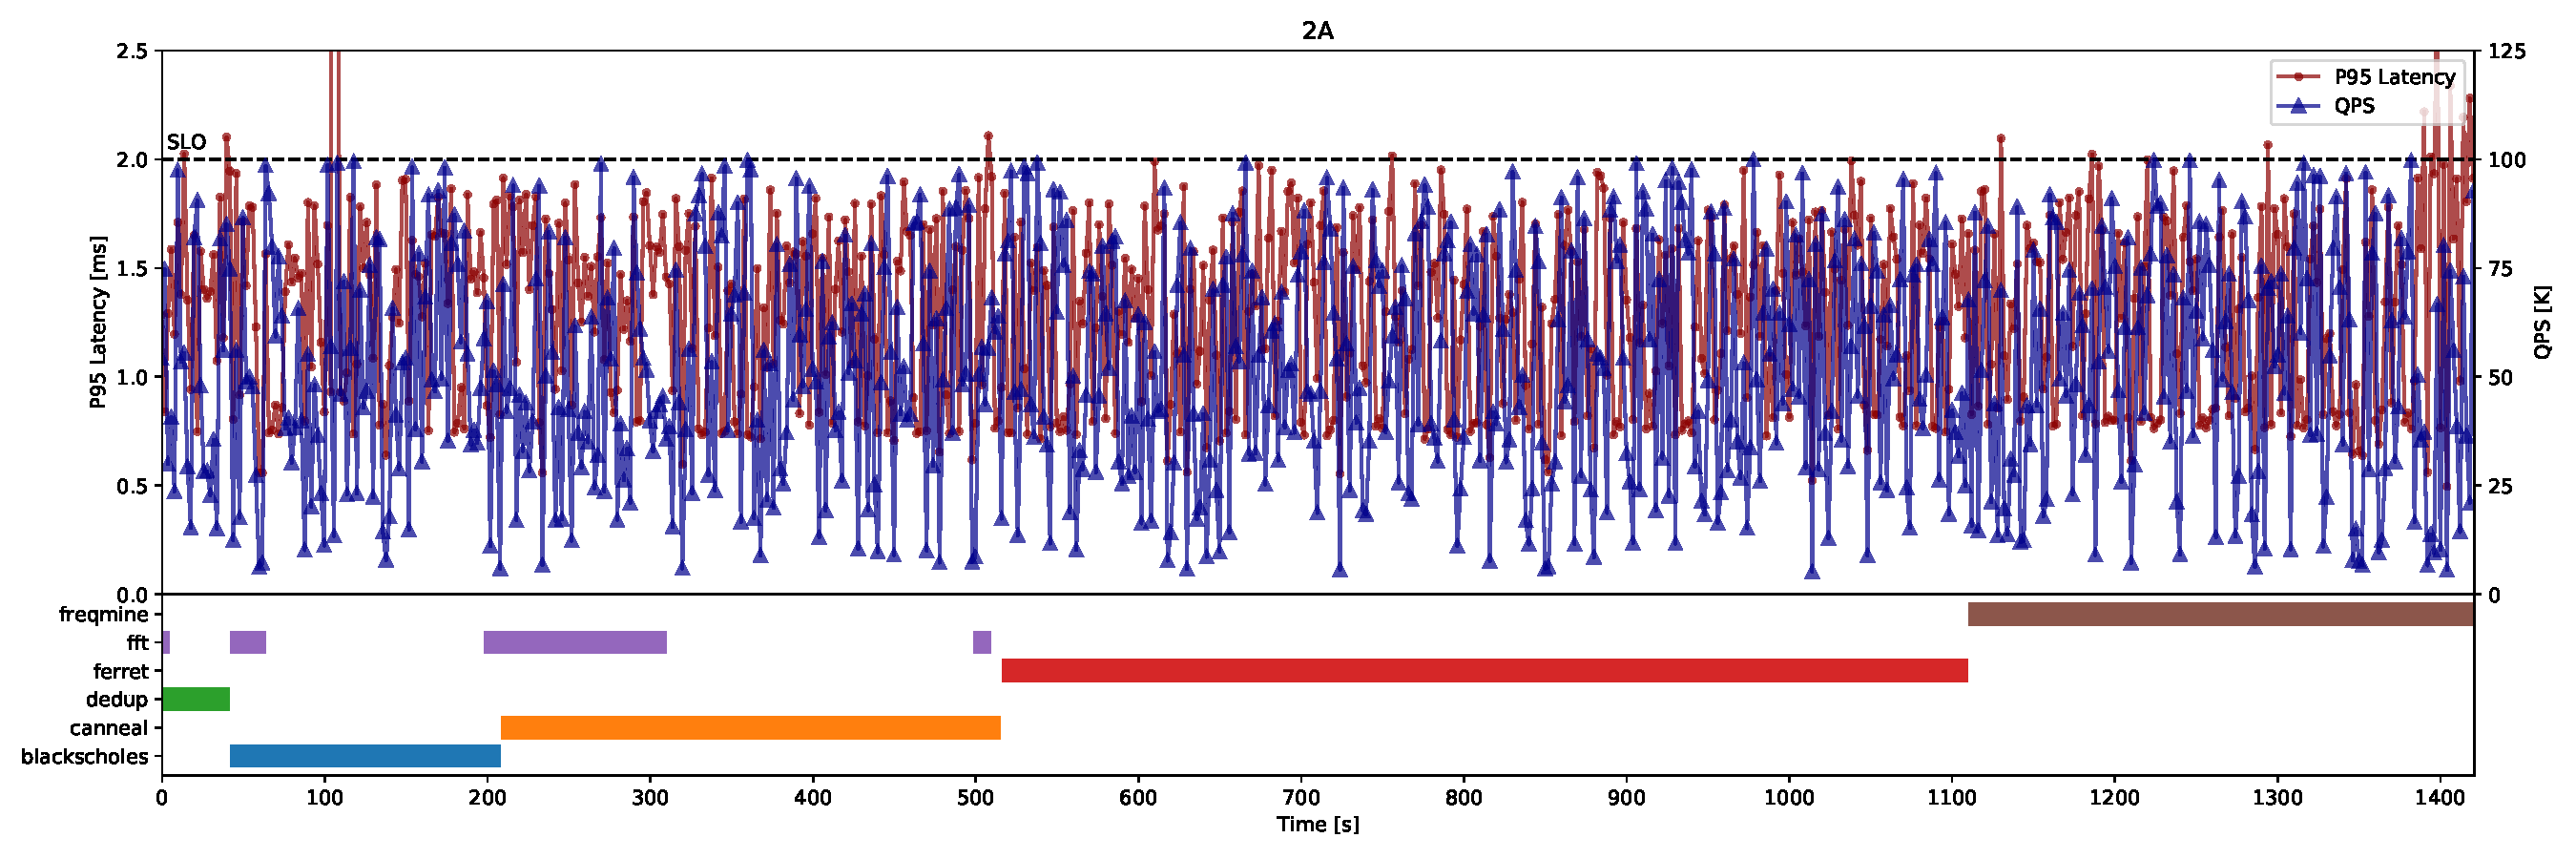
\includegraphics[width=0.9\textwidth]{plot2/2A.pdf}}
    \end{center}
    \begin{center}
    {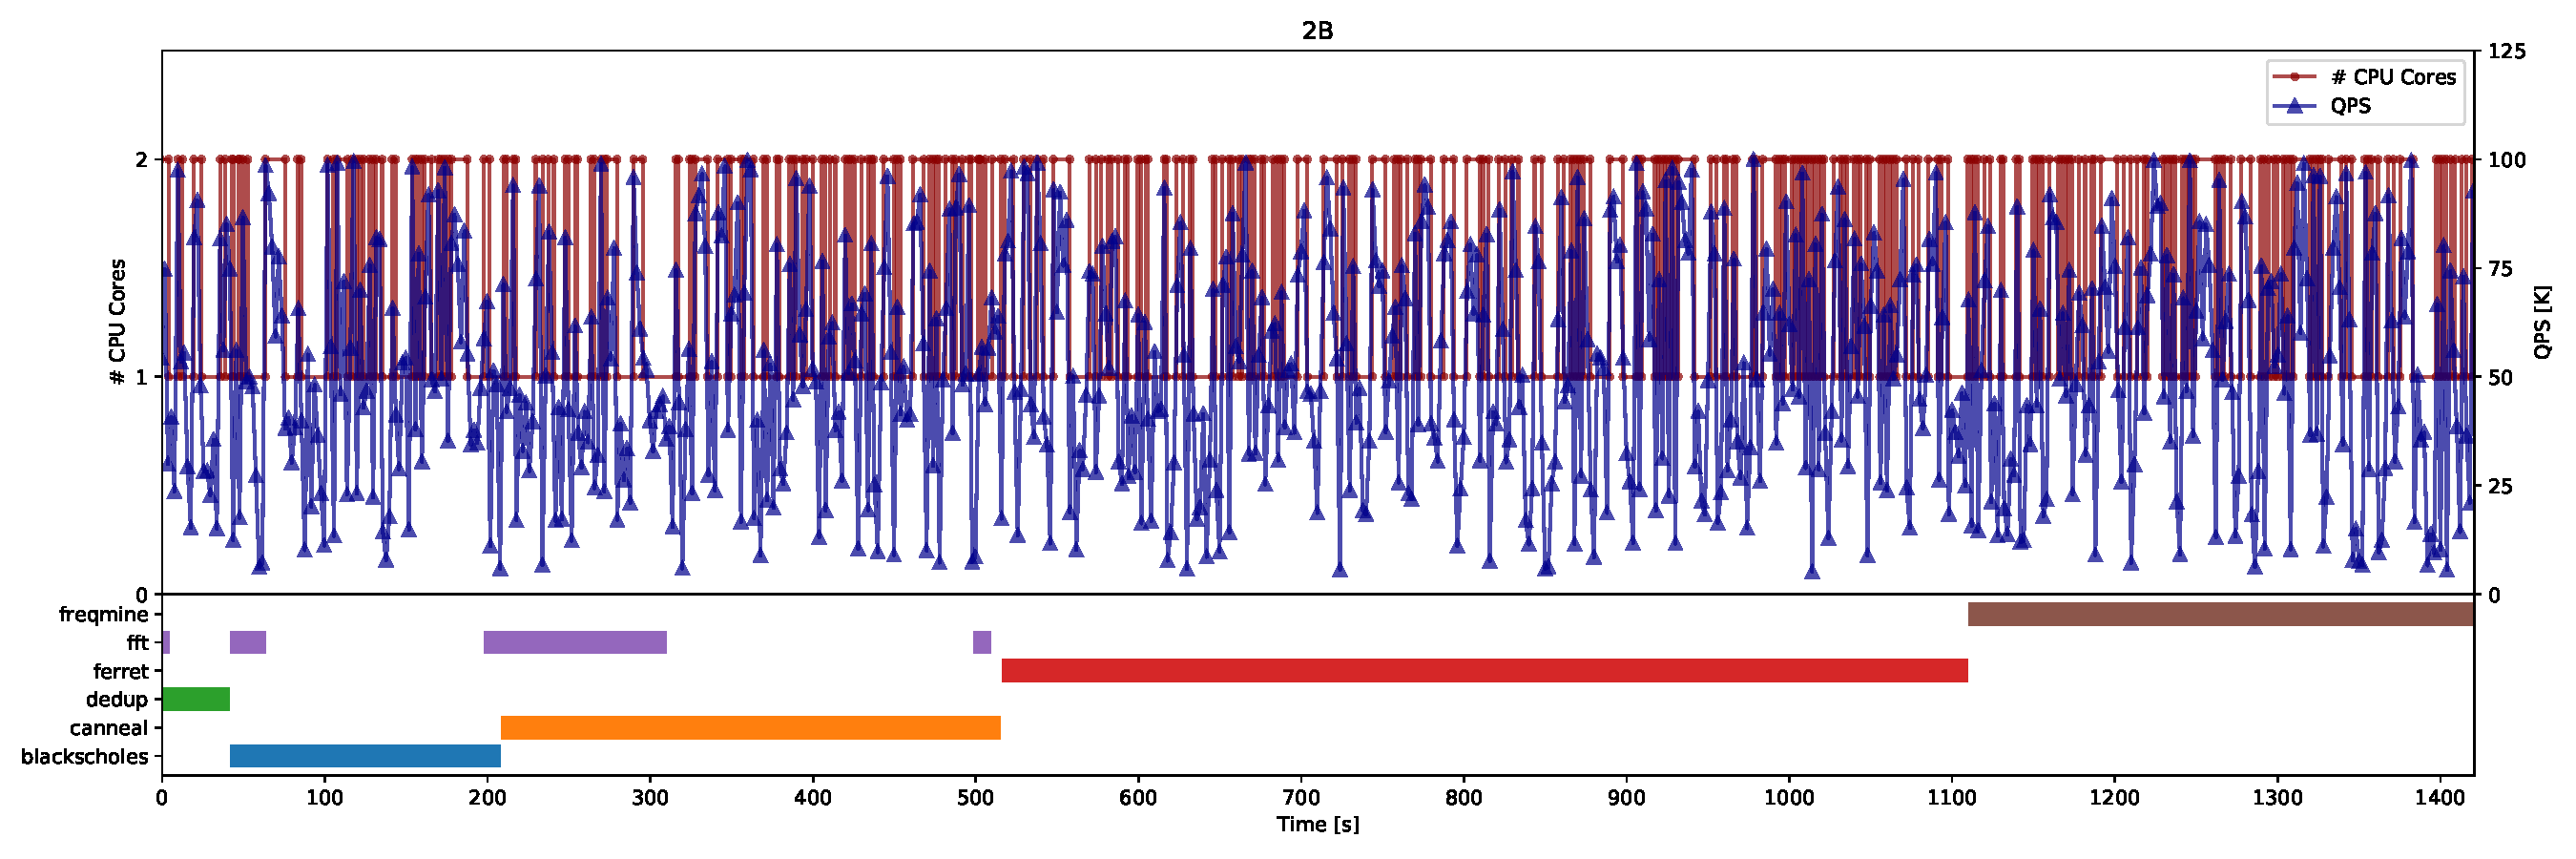
\includegraphics[width=0.9\textwidth]{plot2/2B.pdf}}
    \end{center}
    \begin{center}
    {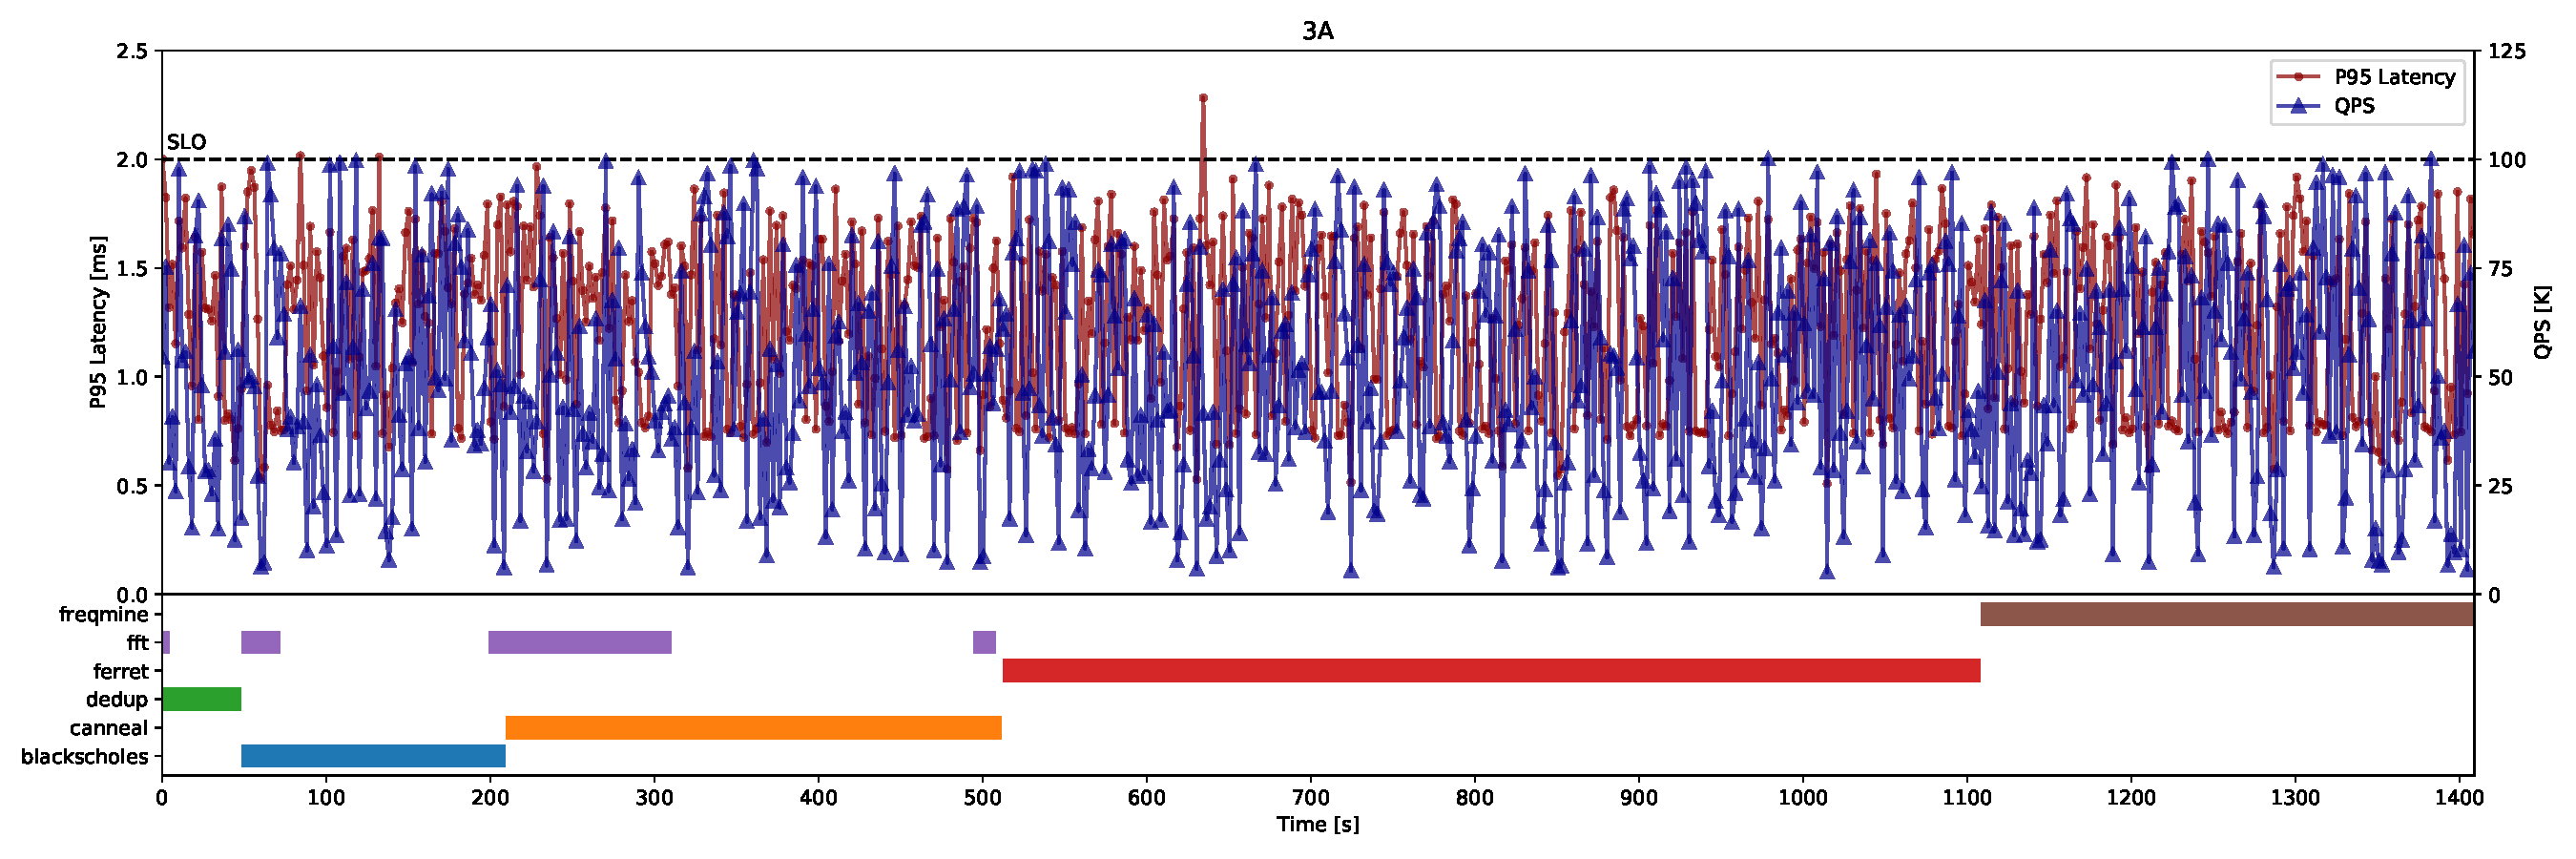
\includegraphics[width=0.9\textwidth]{plot2/3A.pdf}}
    \end{center}
    \begin{center}
    {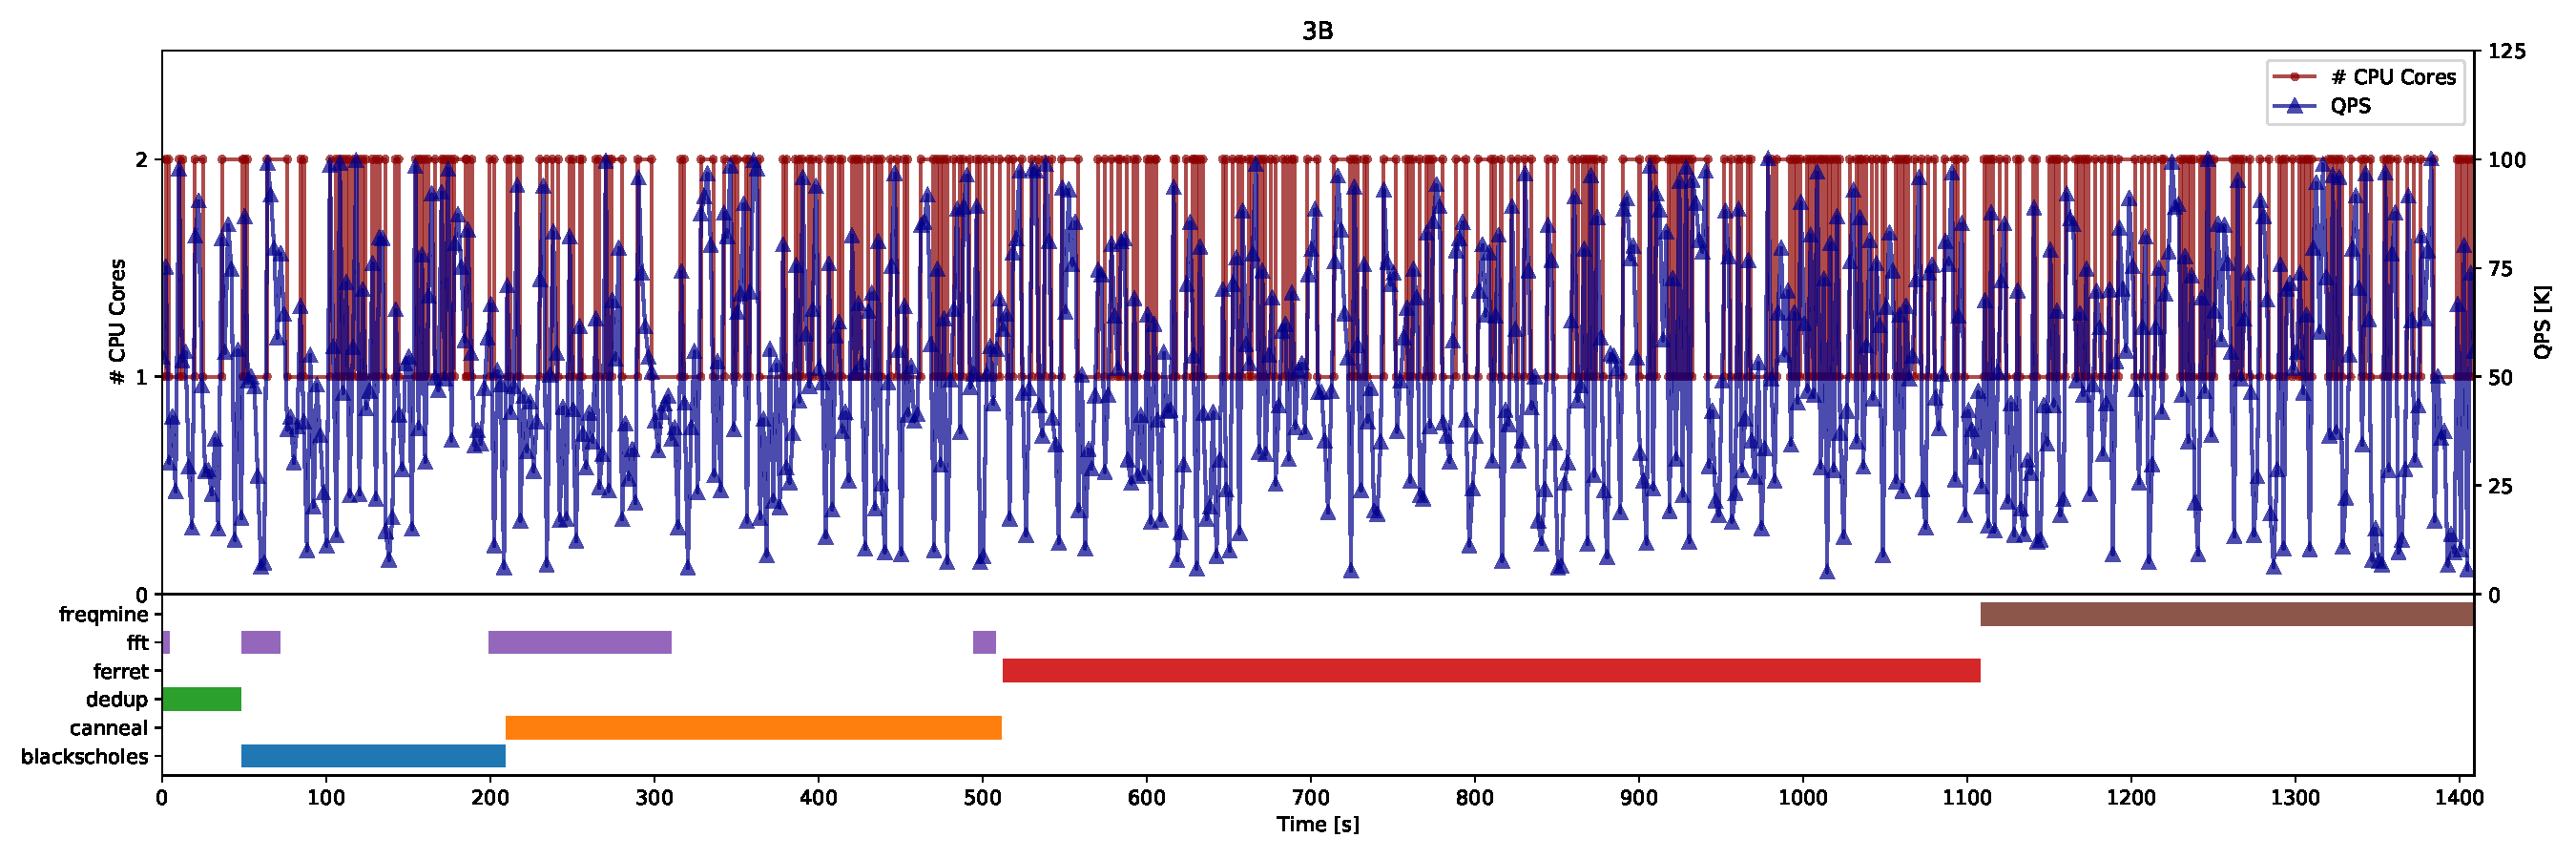
\includegraphics[width=0.9\textwidth]{plot2/3B.pdf}}
    \end{center}
    
\end{enumerate}


\end{document}
